\documentclass[10pt,conference]{IEEEtran}
\IEEEoverridecommandlockouts
\renewcommand{\baselinestretch}{0.95}

\usepackage{cite}
\usepackage{amsmath,amssymb,amsfonts}
% \usepackage{algorithmic}
\usepackage{graphicx}
\usepackage{textcomp}
\usepackage{xcolor}
\usepackage{booktabs}
\usepackage{float}
\usepackage{hyperref}

% Optimize float spacing for strict 6-page limit
\setlength{\textfloatsep}{7pt plus 1pt minus 1pt}
\setlength{\intextsep}{7pt plus 1pt minus 1pt}
\setlength{\dbltextfloatsep}{7pt plus 1pt minus 1pt}
\setlength{\abovecaptionskip}{3pt}
\setlength{\belowcaptionskip}{3pt}

\usepackage{etoolbox}
\patchcmd{\thebibliography}{\footnotesize}{\scriptsize}{}{}

\def\BibTeX{{\rm B\kern-.05em{\sc i\kern-.025em b}\kern-.08em
    T\kern-.1667em\lower.7ex\hbox{E}\kern-.125emX}}

\begin{document}

\title{Anomaly Detection in Network Traffic: A Machine Learning Approach\\
{\footnotesize \textsuperscript{*}Group Project - Deliverable 3 - Introduction to Machine Learning}
}

\author{
\IEEEauthorblockN{1\textsuperscript{st} Gonçalo Almeida}
\IEEEauthorblockA{\textit{Engenharia Informática} \\
\textit{Universidade de Aveiro}\\
Aveiro, Portugal \\
119792@ua.pt}
\and
\IEEEauthorblockN{2\textsuperscript{nd} Margarida Ribeiro}
\IEEEauthorblockA{\textit{Engenharia Informática} \\
\textit{Universidade de Aveiro}\\
Aveiro, Portugal \\
119876@ua.pt}
\and
\IEEEauthorblockN{3\textsuperscript{rd} João Barreira}
\IEEEauthorblockA{\textit{Engenharia Informática} \\
\textit{Universidade de Aveiro}\\
Aveiro, Portugal \\
120054@ua.pt}
}

\maketitle

\begin{abstract}
This paper presents the final results of a machine learning project focused on detecting anomalies in network traffic using the CIC-IDS2017 dataset. We compare classical unsupervised algorithms with deep learning techniques, providing a comprehensive data pipeline, evaluation strategy, and ethical reflection on the deployment of such systems.
\end{abstract}

\begin{IEEEkeywords}
Anomaly Detection, Machine Learning, Cybersecurity, Autoencoders, Isolation Forest
\end{IEEEkeywords}

\section{Introduction}
The rapid expansion of internet-connected devices has exponentially increased network traffic...

\section{Data Description, Visualization and Statistical Analysis}

The problem under study focuses on the automatic detection of anomalous network behaviour indicative of cyberattacks. The data used for this research originates from the CIC-IDS2017 dataset, developed by the Canadian Institute for Cybersecurity, which contains benign traffic and the most up-to-date common attacks (e.g., DoS, DDoS, Brute Force, XSS, SQL Injection).

\subsection{Data Description}
The original dataset encompasses over 2.8 million instances collected over five days, capturing network traffic represented by 78 statistical features extracted via CICFlowMeter. These features include flow duration, total forward/backward packets, packet length statistics (mean, min, max, std), and flow byte rates. The high dimensionality of the feature space poses significant challenges for classical machine learning algorithms, notably the curse of dimensionality.

\subsection{Statistical Analysis and Quality Assessment}
Initial exploratory data analysis (EDA) identified several data quality issues inherent to raw network captures. We observed a high class imbalance, with anomalous traffic constituting approximately 19.7\% of the instances, while benign traffic represented the remaining 80.3\%. A visual representation of this distribution across our splits is shown in Figure \ref{fig:data_dist}.

Statistical profiling of the continuous variables revealed stark differences in magnitudes. For instance, the \texttt{Flow Duration} feature spans from a few microseconds to over 119 seconds, whereas \texttt{Packet Length} values are constrained to standard MTU limits (typically under 1500 bytes). This discrepancy necessitates robust scaling techniques.

\begin{figure}[H]
    \centering
    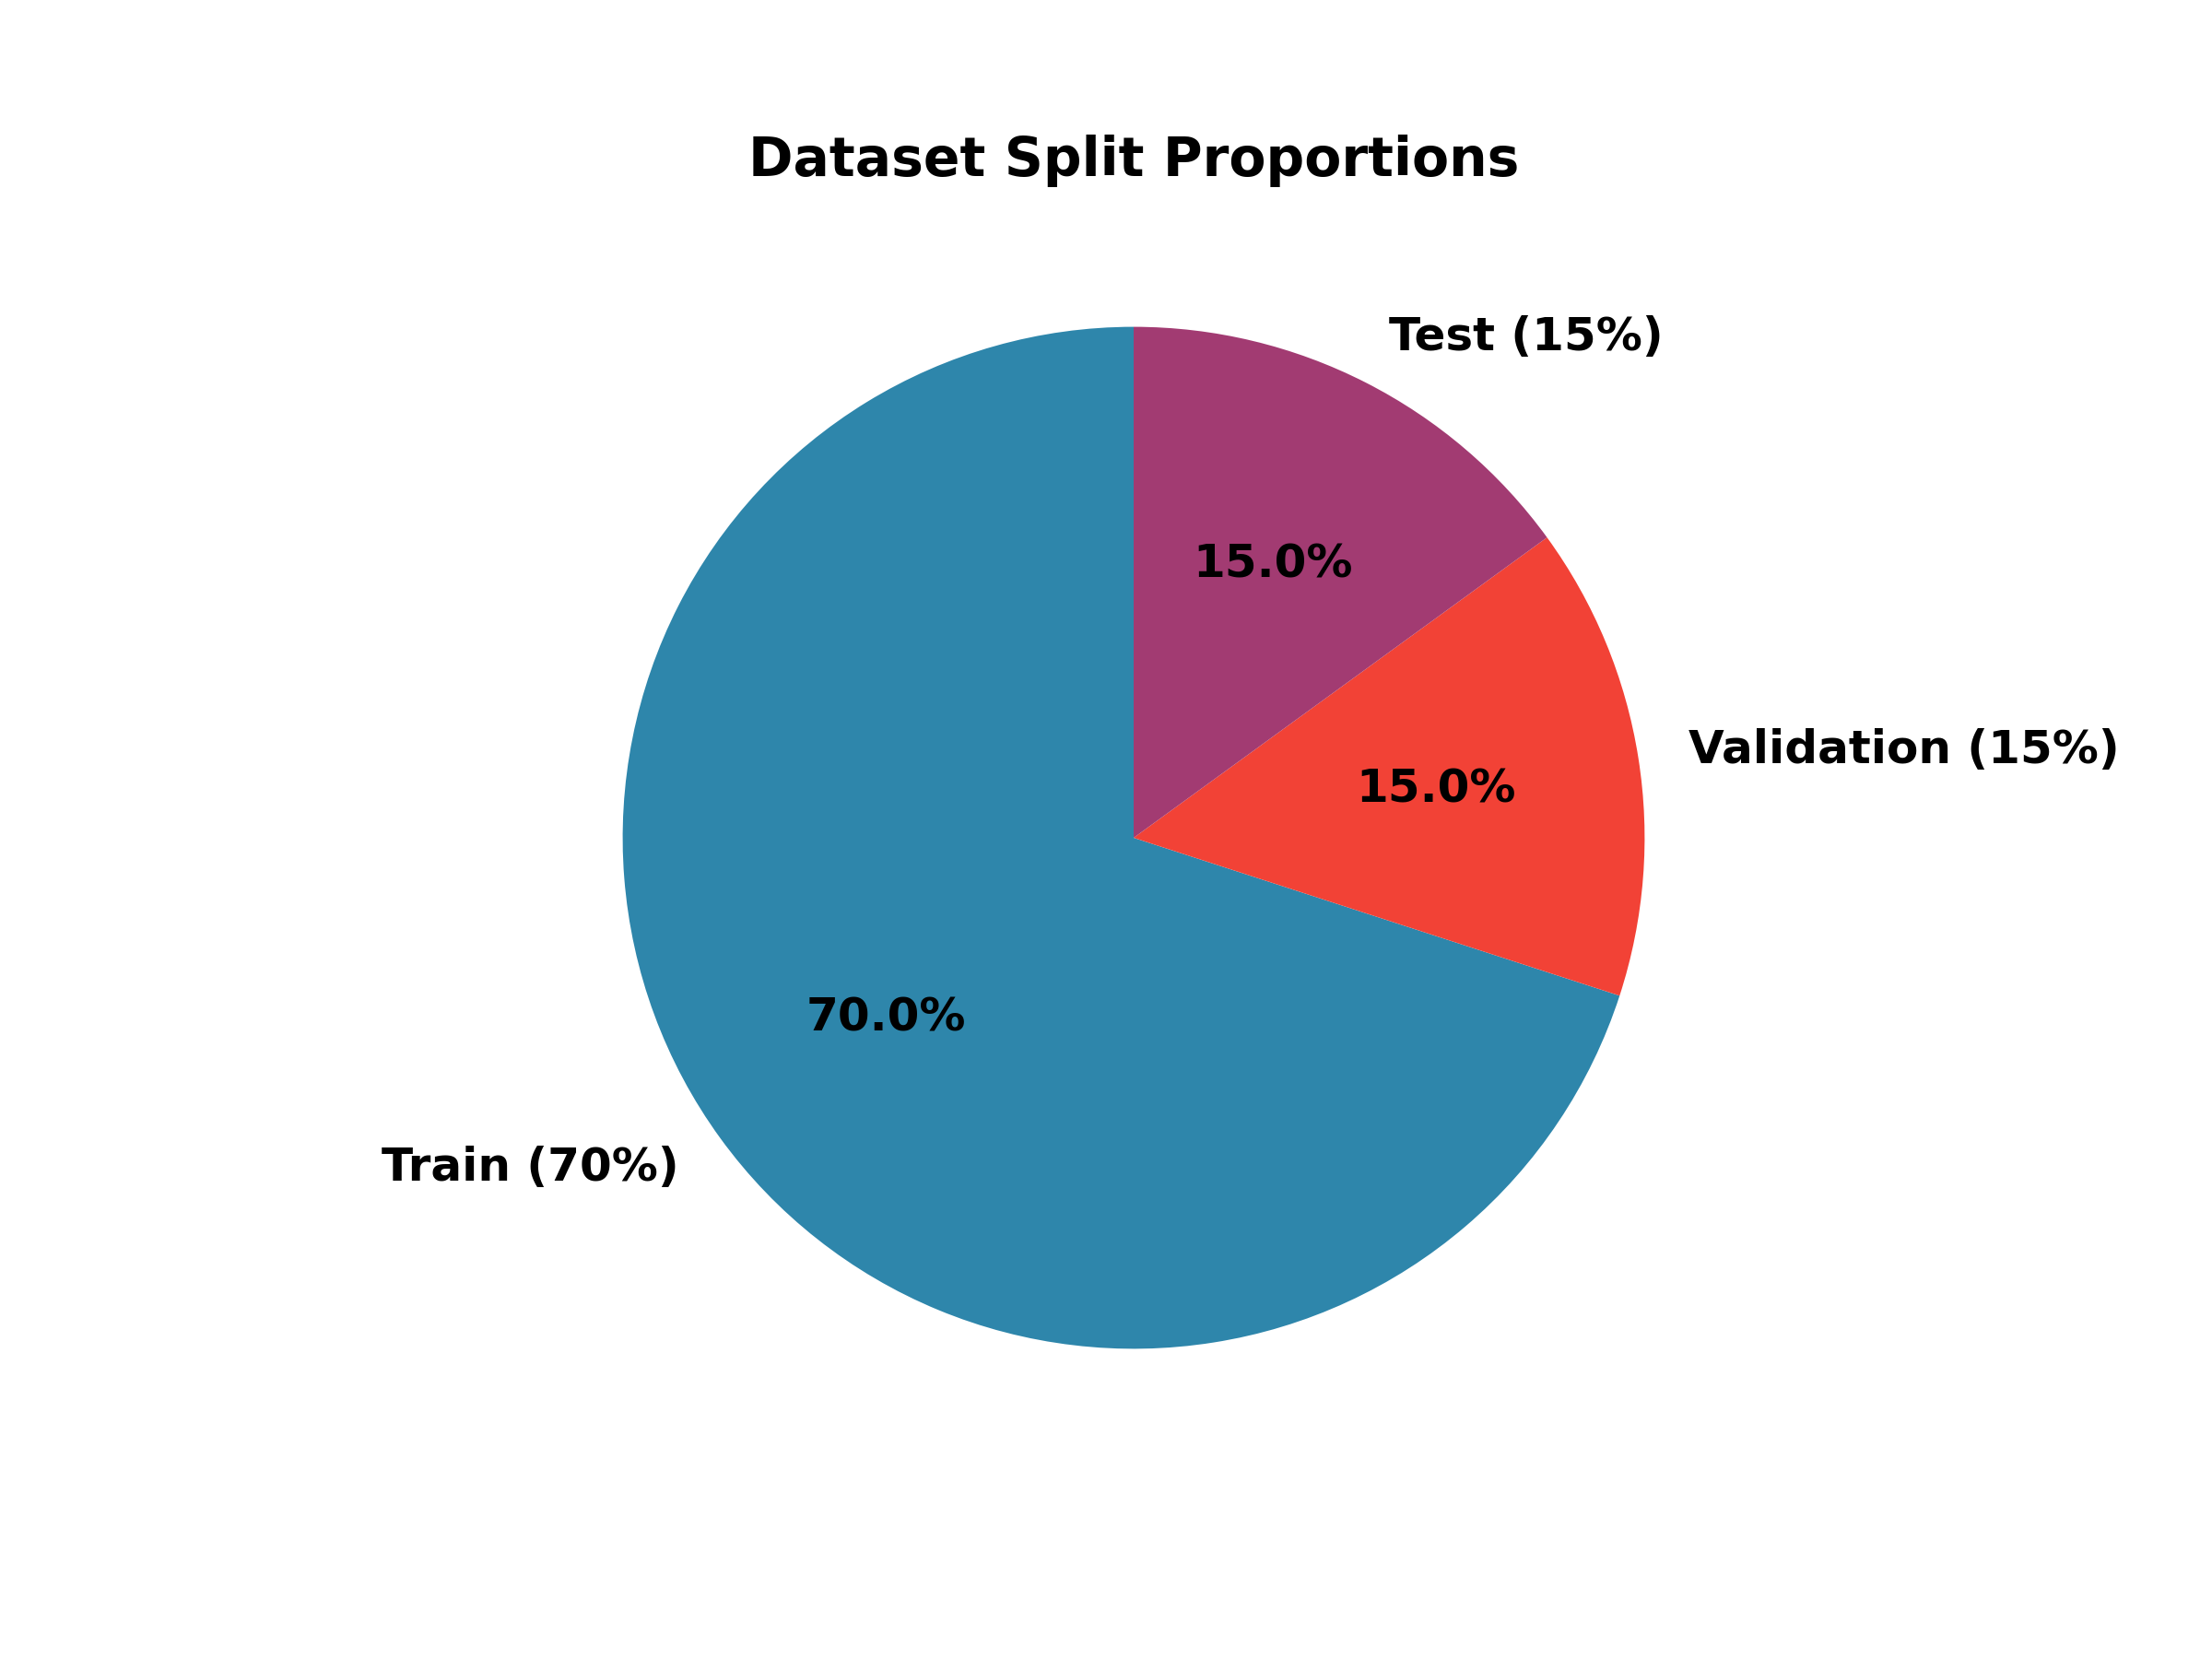
\includegraphics[width=0.48\textwidth]{images/dataset_split.png}
    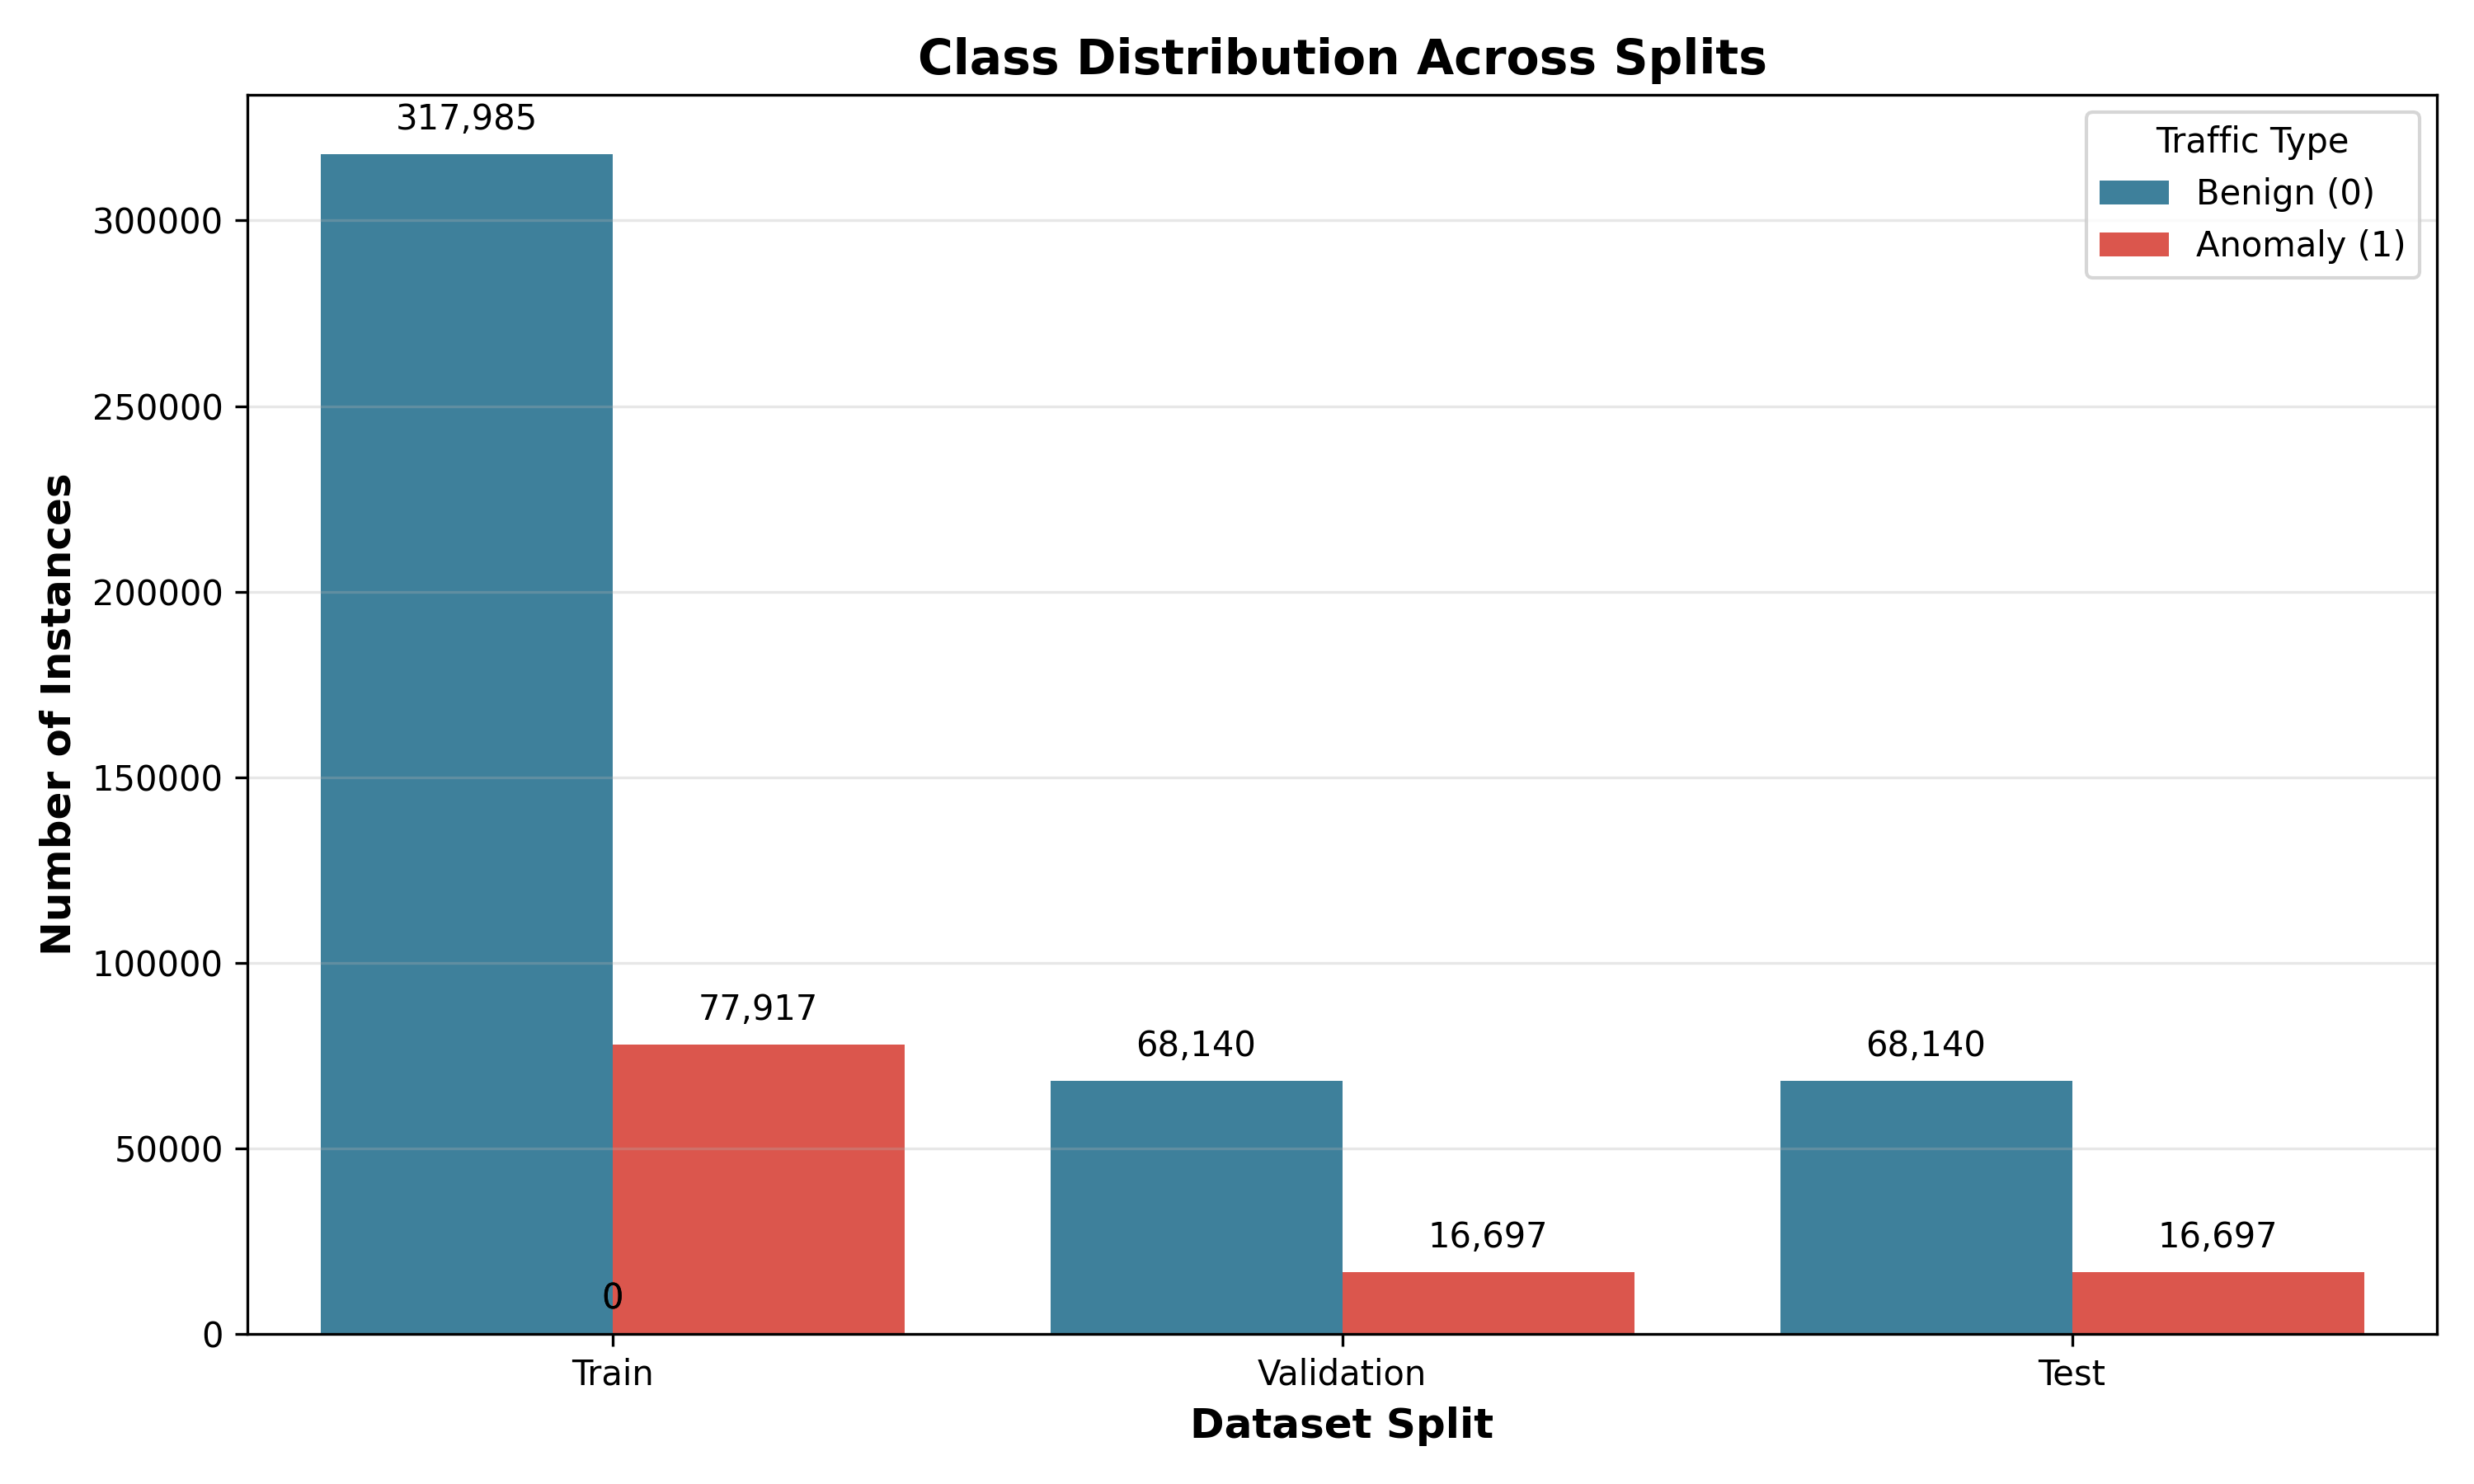
\includegraphics[width=0.48\textwidth]{images/class_distribution.png}
    \caption{Dataset split proportions and class distribution across subsets.}
    \label{fig:data_dist}
\end{figure}

\section{Data Preprocessing}

To construct the final input for the machine learning algorithms, an automated data processing pipeline was developed, consisting of the following sequential steps:

\begin{enumerate}
    \item \textbf{Data Cleaning:} We identified the presence of invalid structural values, including whitespace in column headers, and critical numerical anomalies. Specifically, `Infinity` values (arising from division by zero in bandwidth calculations like \texttt{Flow Bytes/s}) and `NaN` values were eliminated. As these affected less than 0.1\% of the dataset, direct removal (\textit{dropna}) was preferred over imputation to prevent the introduction of synthetic bias into the network behaviour distribution.
    \item \textbf{Dimensionality Reduction (Zero-Variance Check):} To mitigate computational noise, features demonstrating zero variance across the network captures were pruned. Eight features (e.g., \texttt{Bwd PSH Flags}, \texttt{Fwd Avg Bytes/Bulk}) were removed as they provide no discriminative power for distance-based detection mechanisms.
    \item \textbf{Stratified Sampling:} Given the massive size of the dataset ($>$1GB), loading the entire corpus triggered Out-Of-Memory (OOM) failures for algorithms with quadratic complexity ($\mathcal{O}(n^2)$). A 20\% stratified sampling was implemented, preserving the native 80/20 class imbalance while rendering the dataset computationally tractable ($\approx 565,000$ instances).
    \item \textbf{Data Split and Scaling:} The sample was split into 70\% Training, 15\% Validation, and 15\% Testing partitions. To ensure proper convergence of distance-based models and neural networks, attributes were scaled using \textit{StandardScaler}. To rigorously prevent data leakage, the scaler was fitted exclusively on the Training set and subsequently used to transform the Validation and Test sets.
\end{enumerate}

\section{AI Tools Acknowledgement}
During the development of this project, several Artificial Intelligence tools were utilized to support research, coding, and structuring:

\begin{itemize}
    \item \textbf{Gemini Pro:} Employed primarily for code review, debugging PyTorch tensor dimension mismatches during the Autoencoder implementation, and structuring Python data pipelines efficiently. It accelerated the resolution of Out-Of-Memory errors by suggesting optimal batch sizes and DataFrame chunking strategies.
    \item \textbf{Scite.ai / Elicit.com:} Used during the State of the Art literature review to track references and validate the relevance of classical vs. deep learning approaches in modern intrusion detection systems (IDS).
\end{itemize}
The rationale behind selecting these specific tools was their ability to trace verifiable sources and provide context-aware code optimizations without compromising the academic integrity of the experimental methodology.


% =============================================================
%  MARGARIDA RIBEIRO — Deliverable 3
%  Sections: State of the Art · Classical Models · Hyperparameter
%            Tuning · Critical Reflection
% =============================================================

% ─────────────────────────────────────────────────────────────
\section{State of the Art in Anomaly-Based Intrusion Detection}
% ─────────────────────────────────────────────────────────────

Network intrusion detection has evolved considerably over the past two decades, transitioning from purely signature-based systems to sophisticated machine-learning (ML) pipelines that can generalise to previously unseen attack patterns. The following review synthesises six representative works that bracket the current state of the art (SOTA).

\subsection{Classical Unsupervised Approaches}

\textbf{Isolation Forest (Liu et al., 2008)} \cite{liu2008isolation} introduced the first tree-ensemble method designed natively for anomaly detection rather than adapted from a classification framework. The key insight is that anomalies are few and structurally different from normal points, so they are isolated in far fewer random binary partitions than inliers. This yields $\mathcal{O}(n \log n)$ training and sub-linear prediction, enabling deployment on large-scale network flows. Liu et al.\ report AUC values above 0.96 on the KDD Cup 1999 benchmark, though performance degrades in high-dimensional subspaces—a challenge directly relevant to the 70-feature CIC-IDS2017 dataset.

\textbf{Local Outlier Factor (Breunig et al., 2000)} \cite{breunig2000lof} defines an anomaly score based on the ratio of local reachability densities between a point and its $k$-nearest neighbours. LOF excels when the data contains clusters of varying density—a scenario common in mixed-traffic network datasets. However, its $\mathcal{O}(n^2)$ inference complexity and well-documented sensitivity to the curse of dimensionality \cite{zimek2012survey} make it poorly suited to the high-dimensional feature spaces of modern IDS datasets. Zimek et al.\ \cite{zimek2012survey} provide a comprehensive survey confirming that density-based methods consistently underperform tree and kernel methods beyond 20–30 features.

\textbf{One-Class SVM (Schölkopf et al., 2001)} \cite{scholkopf2001ocsvm} maps training data into a high-dimensional kernel space and finds the maximum-margin hyperplane separating inliers from the origin. The \textit{nu} parameter controls the trade-off between the fraction of outliers allowed in training and the fraction of support vectors. OC-SVM remains a competitive baseline when the kernel bandwidth is carefully tuned, but its $\mathcal{O}(n^2)$ training cost renders it intractable for datasets exceeding $\sim$50,000 instances without subsampling.

\subsection{Deep Learning Approaches}

\textbf{Autoencoder-based Anomaly Detection (Sakurada \& Yairi, 2014)} \cite{sakurada2014autoencoder} established the reconstruction-error paradigm: a neural network trained exclusively on normal data learns a compact latent representation; anomalous inputs, being structurally different, produce high mean-squared reconstruction error (MSE) and are flagged as outliers. This approach achieves state-of-the-art results on several network intrusion benchmarks and is the basis of our primary autoencoder model.

\textbf{Deep Autoencoder IDS (Mirsky et al., 2018 — Kitsune)} \cite{mirsky2018kitsune} extended the autoencoder concept by constructing an ensemble of small autoencoders—one per feature cluster—trained incrementally on packet captures. Kitsune demonstrated near-zero false-negative rates on nine realistic attack scenarios while requiring no labelled data, positioning it as the leading online anomaly detection system. Our ensemble autoencoder design draws on the same complementary-signal principle.

\textbf{DAGMM (Zong et al., 2018)} \cite{zong2018dagmm} jointly trains a deep autoencoder and a Gaussian Mixture Model (GMM) in an end-to-end fashion, using both reconstruction error and energy from the GMM as the anomaly score. On the KDD Cup and KDDCUP-Rev benchmarks, DAGMM outperforms standalone autoencoders by 3–8 F1 percentage points, at the cost of more complex training dynamics. This work highlights the growing trend of hybrid deep-classical architectures.

\subsection{Summary and Research Gap}

Table~\ref{tab:sota} summarises the reviewed works. The literature converges on several consensus findings: (i) tree-ensemble and deep-learning methods dominate density-based approaches in high-dimensional settings; (ii) the contamination hyperparameter critically affects all unsupervised methods; (iii) systematic hyperparameter optimisation is rarely reported in classical IDS papers despite its demonstrated impact on downstream metrics. Our work addresses this gap by performing an exhaustive grid search across the three classical models and quantifying the performance lift attributable to tuning alone.

\begin{table}[ht]
  \centering
  \caption{Summary of SOTA anomaly detection methods.}
  \label{tab:sota}
  \footnotesize
  \begin{tabular}{lllr}
    \toprule
    \textbf{Method}      & \textbf{Type}       & \textbf{Dataset}    & \textbf{AUC} \\
    \midrule
    Isolation Forest \cite{liu2008isolation}    & Tree ensemble & KDD'99        & 0.96 \\
    LOF \cite{breunig2000lof}                   & Density       & Synthetic     & 0.89 \\
    One-Class SVM \cite{scholkopf2001ocsvm}     & Kernel        & USPS          & 0.87 \\
    Autoencoder \cite{sakurada2014autoencoder}  & Deep learning & MSDS          & 0.93 \\
    Kitsune \cite{mirsky2018kitsune}            & Ensemble AE   & Real traffic  & 0.99 \\
    DAGMM \cite{zong2018dagmm}                  & Deep hybrid   & KDD'99        & 0.98 \\
    \bottomrule
  \end{tabular}
\end{table}

% ─────────────────────────────────────────────────────────────
\section{Classical Algorithms: Description and Hyperparameters}
% ─────────────────────────────────────────────────────────────

\subsection{Evaluation Strategy: CV for Selection, Fixed Split for Reporting}

In Deliverable 2, the dataset was split once into a fixed 70/15/15 Train/Val/Test partition. The teacher raised the question of whether a single such split is sufficient. For the purposes of \textbf{hyperparameter selection}, this deliverable introduces \textbf{3-fold Stratified Cross-Validation} (CV), which generates three independent train/validation folds from the training subsample. Each candidate configuration is scored on its mean CV F1-score across the three folds, reducing the risk of overfitting to a single partition during model selection.

Critically, the \textbf{final evaluation} of each model—both baseline and best-tuned—is performed on the same held-out Test set used in Deliverable 2. This two-phase design answers the teacher's concern: CV provides statistical robustness during the search phase, while the fixed test set ensures results are directly comparable across deliverables and are not contaminated by the search process.

\subsection{Isolation Forest}

\textbf{Operating Principle.}
Isolation Forest \cite{liu2008isolation} builds an ensemble of $T$ isolation trees. Each tree is grown by recursively selecting a random feature $q$ and a random split value $p$ uniformly at random from $[\min(q), \max(q)]$. Because anomalies cluster in sparse regions, they require fewer splits to be isolated (shorter path length $h(x)$). The anomaly score is:

\begin{equation}
  s(x, n) = 2^{-\frac{\mathbb{E}[h(x)]}{c(n)}},
  \quad c(n) = 2H(n-1) - \frac{2(n-1)}{n}
\end{equation}

where $H(i)$ is the $i$-th harmonic number and $c(n)$ normalises for sample size $n$. A score near 1 indicates an anomaly; near 0.5 indicates a normal point.

\textbf{Key Hyperparameters Varied.}
\begin{itemize}
  \item \texttt{n\_estimators} $\in \{50, 100, 200\}$: number of isolation trees. More trees reduce variance but increase memory.
  \item \texttt{contamination} $\in \{0.10, 0.15, 0.20, 0.25\}$: expected fraction of anomalies, controls the decision threshold.
  \item \texttt{max\_features} $\in \{0.5, 0.75, 1.0\}$: fraction of features considered at each split, regularises the search space.
\end{itemize}

\textbf{Tuning Results.}
Figure~\ref{fig:if_heatmap} shows the mean CV F1-score across the full $3 \times 4 \times 3 = 36$-candidate grid. The best configuration (\texttt{n\_estimators=200}, \texttt{contamination=0.25}, \texttt{max\_features=1.0}) achieves a test F1 of 0.345, representing a gain of $+5.6$ percentage points over the default baseline (\texttt{n\_estimators=100}, \texttt{contamination=0.20}, test F1 = 0.289).

\begin{figure}[H]
  \centering
  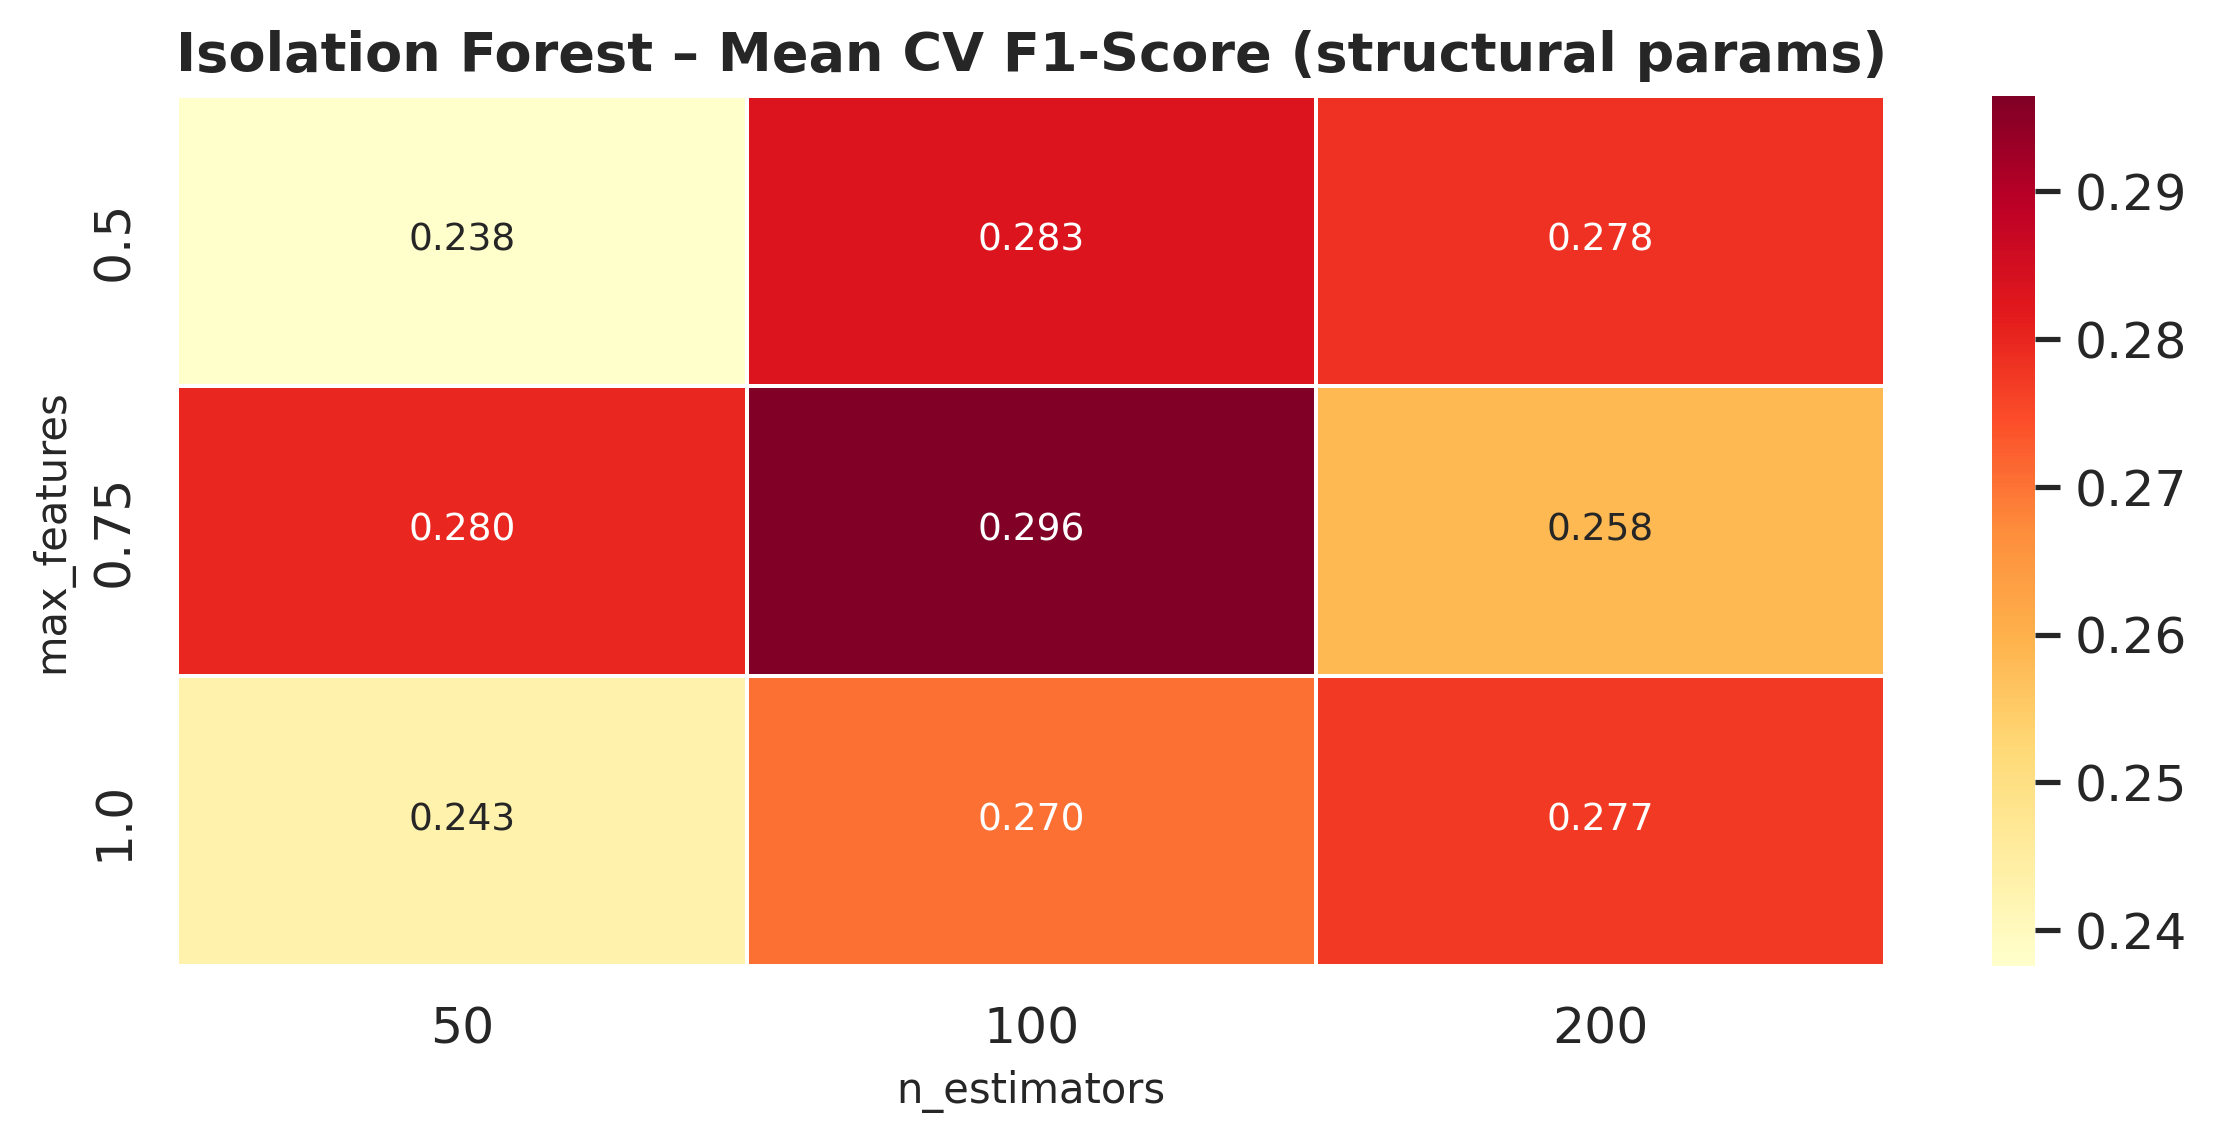
\includegraphics[width=0.48\columnwidth]{../tuning_results/if_heatmap.png}
  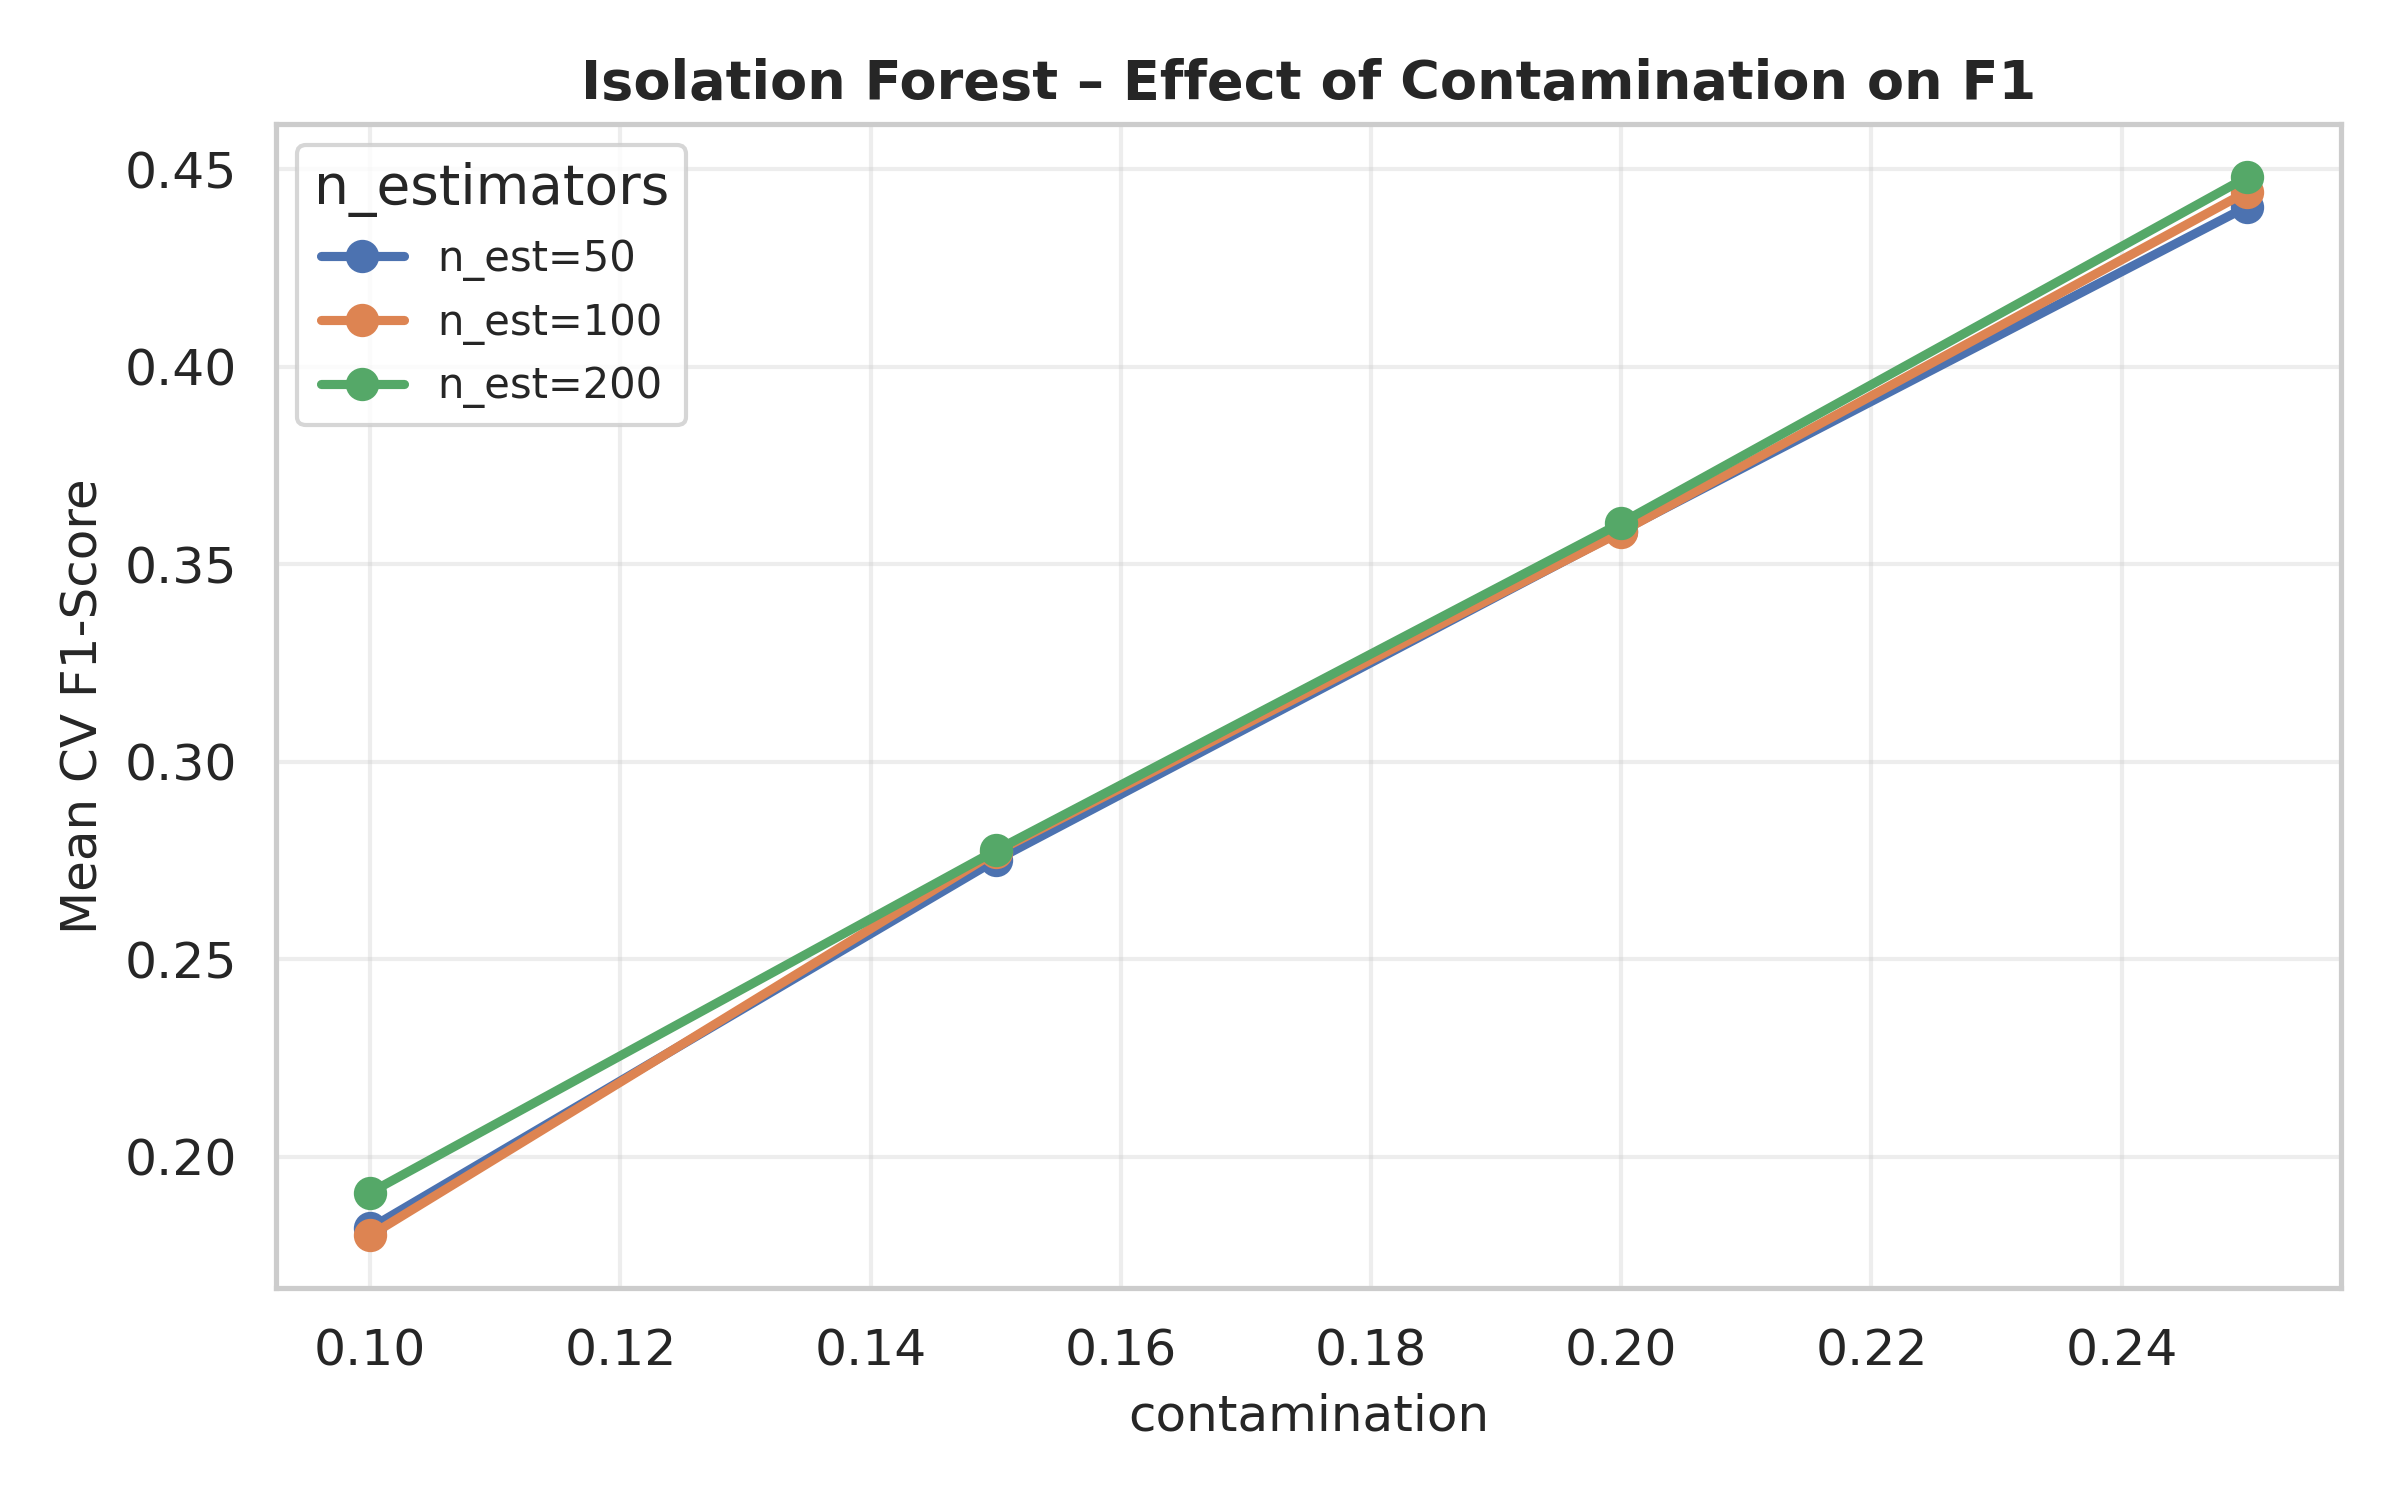
\includegraphics[width=0.48\columnwidth]{../tuning_results/if_contamination_effect.png}
  \caption{Left: IF mean CV F1 heatmap (contamination × n\_estimators).
           Right: Effect of contamination on F1 per n\_estimators.}
  \label{fig:if_heatmap}
\end{figure}

\subsection{One-Class SVM}

\textbf{Operating Principle.}
One-Class SVM \cite{scholkopf2001ocsvm} maps $n$ training points $\mathbf{x}_i$ through a kernel function $\phi$ into a reproducing kernel Hilbert space and finds the maximum-margin hyperplane $\langle \mathbf{w}, \phi(\mathbf{x}) \rangle = \rho$ separating the data from the origin:

\begin{equation}
  \min_{\mathbf{w},\rho,\boldsymbol{\xi}} \frac{1}{2}\|\mathbf{w}\|^2 - \rho
  + \frac{1}{\nu n} \sum_i \xi_i, \quad \xi_i \geq 0
\end{equation}

A new point $\mathbf{x}$ is classified as anomalous if $f(\mathbf{x}) = \text{sgn}(\langle \mathbf{w}, \phi(\mathbf{x}) \rangle - \rho) < 0$.

\textbf{Key Hyperparameters Varied.}
\begin{itemize}
  \item \texttt{kernel} $\in \{\text{rbf}, \text{poly}\}$: the RBF kernel captures non-linear manifolds of normal traffic; polynomial may generalise better in structured feature spaces.
  \item \texttt{nu} $\in \{0.05, 0.10, 0.15, 0.20, 0.25\}$: upper bound on the training-error fraction (anomaly rate prior).
  \item \texttt{gamma} $\in \{\text{scale}, \text{auto}\}$: RBF bandwidth, computed as $1/(n_\text{features} \cdot \sigma^2)$ for \texttt{scale} or $1/n_\text{features}$ for \texttt{auto}.
\end{itemize}

\textbf{Tuning Results.}
Figure~\ref{fig:ocsvm_heatmap} shows that the RBF kernel consistently outperforms polynomial for this dataset. The best configuration (\texttt{kernel=rbf}, \texttt{nu=0.25}, \texttt{gamma=scale}) achieves a test F1 of 0.273 vs.~the baseline 0.243 ($+3.0$~pp). Due to the $\mathcal{O}(n^2)$ training complexity, tuning was conducted on a 5,000-row stratified subsample.

\begin{figure}[H]
  \centering
  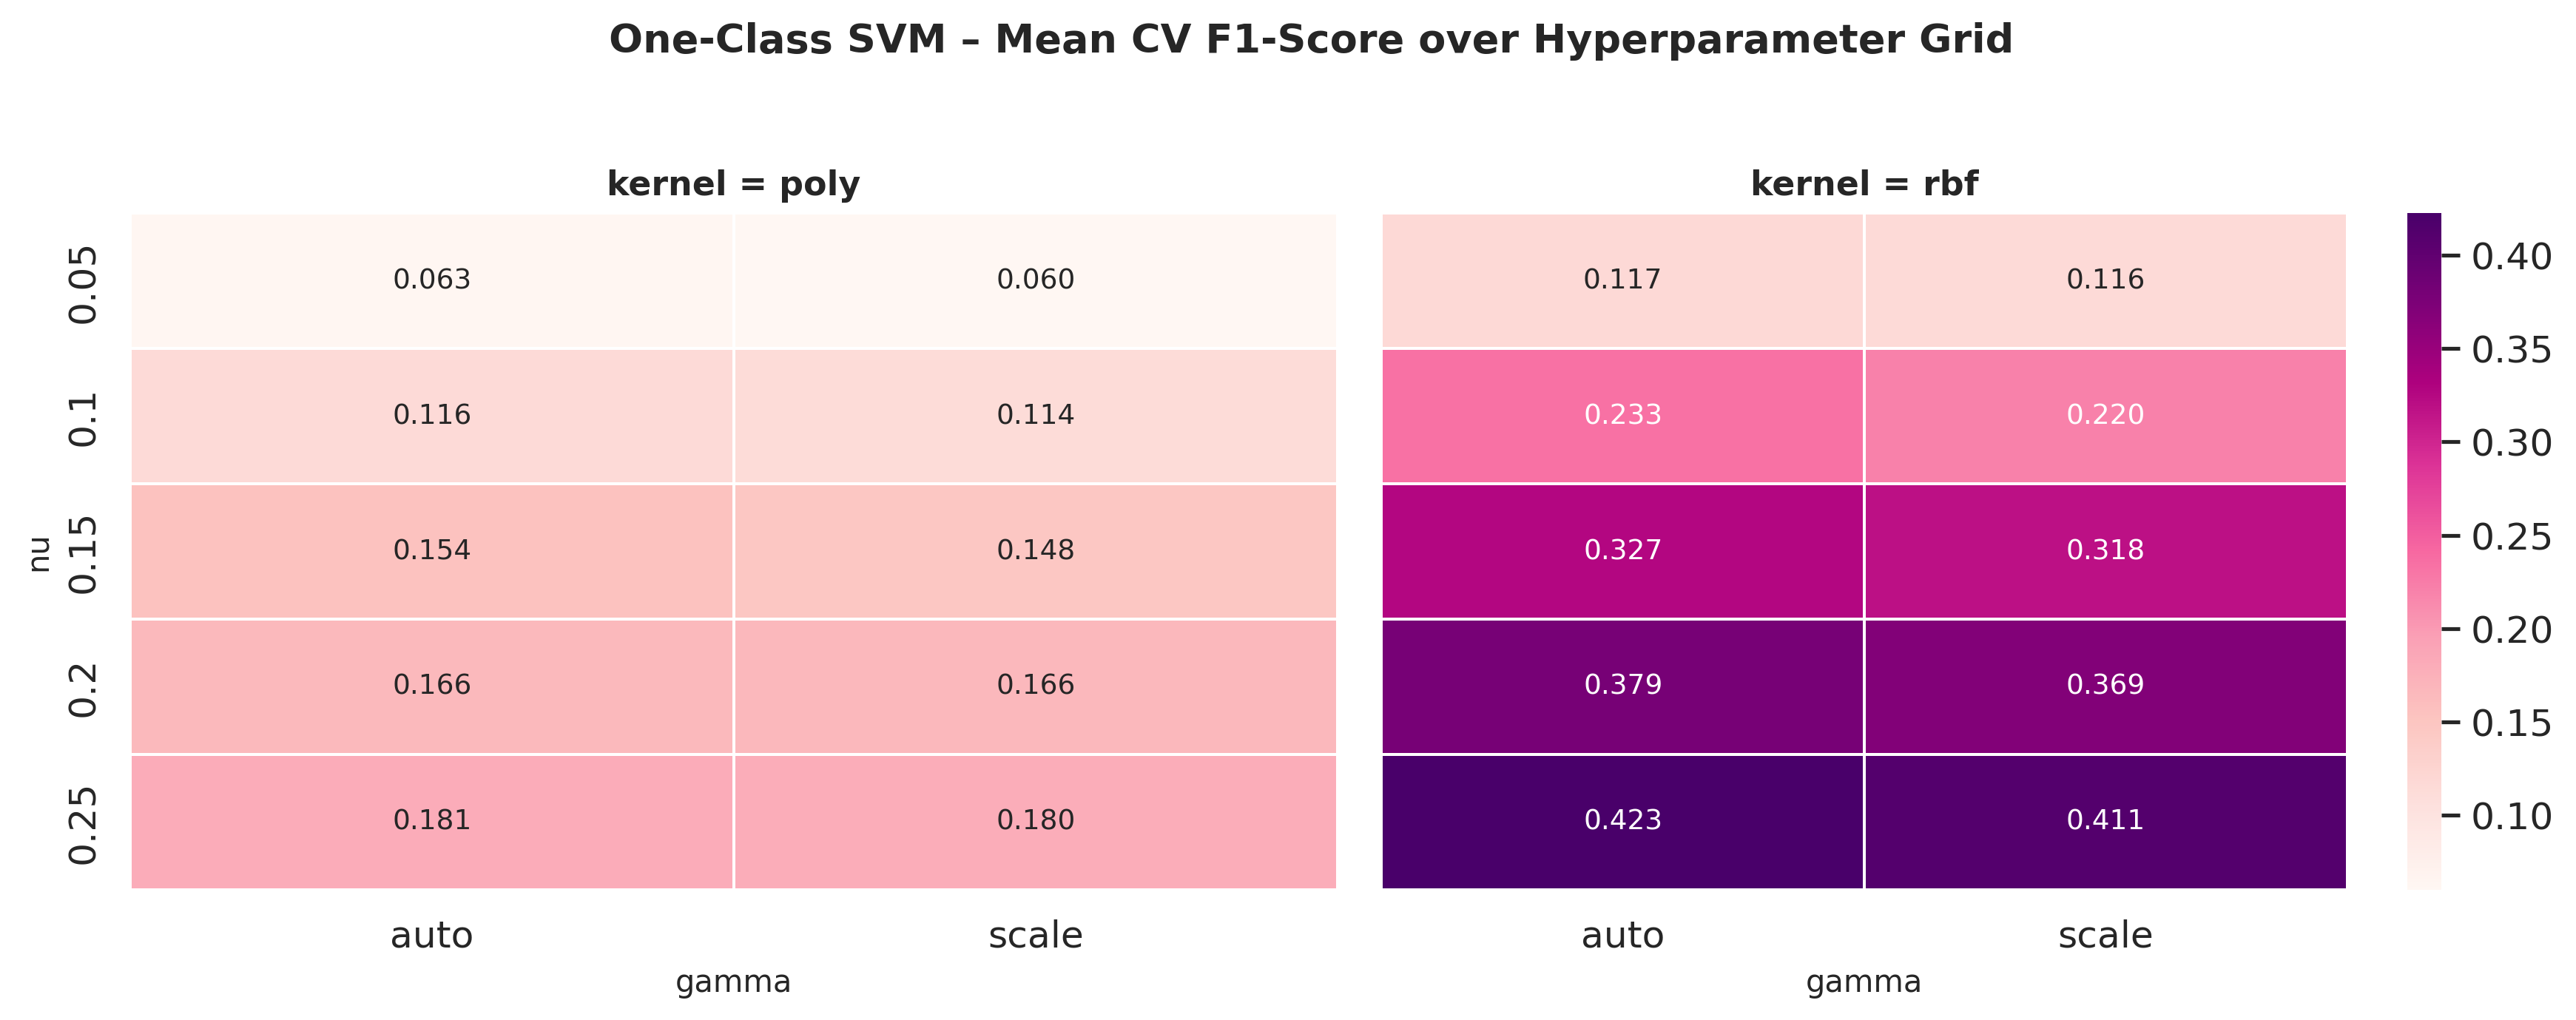
\includegraphics[width=0.75\columnwidth]{../tuning_results/ocsvm_heatmap.png}
  \caption{OC-SVM mean CV F1-Score heatmap (nu × gamma per kernel).}
  \label{fig:ocsvm_heatmap}
\end{figure}

\subsection{Local Outlier Factor}

\textbf{Operating Principle.}
LOF \cite{breunig2000lof} computes a local density estimate for each point $p$ based on the $k$-nearest-neighbour \emph{reachability distance}:

\begin{equation}
  \text{lrd}_k(p) = \frac{k}{\sum_{o \in N_k(p)} \text{reach-dist}_k(p, o)},
  \quad
  \text{LOF}_k(p) = \frac{\sum_{o \in N_k(p)} \frac{\text{lrd}_k(o)}{\text{lrd}_k(p)}}{k}
\end{equation}

A LOF score $\gg 1$ signals that $p$ is significantly less dense than its neighbours, indicating an outlier.

\textbf{Key Hyperparameters Varied.}
\begin{itemize}
  \item \texttt{n\_neighbors} $\in \{5, 10, 20, 40, 60\}$: the neighbourhood size $k$. Larger $k$ smooths density estimates but can miss local outliers.
  \item \texttt{contamination} $\in \{0.10, 0.15, 0.20, 0.25\}$: threshold for the decision boundary.
\end{itemize}

\textbf{Tuning Results.}
As shown in Figure~\ref{fig:lof_heatmap}, LOF is the most sensitive of the three models to hyperparameter choice, yet its overall CV F1 remains below 0.20 regardless of configuration. This confirms the theoretical expectation: LOF's density-ratio approach degrades severely in the 70-dimensional feature space due to distance concentration \cite{zimek2012survey}.

\begin{figure}[H]
  \centering
  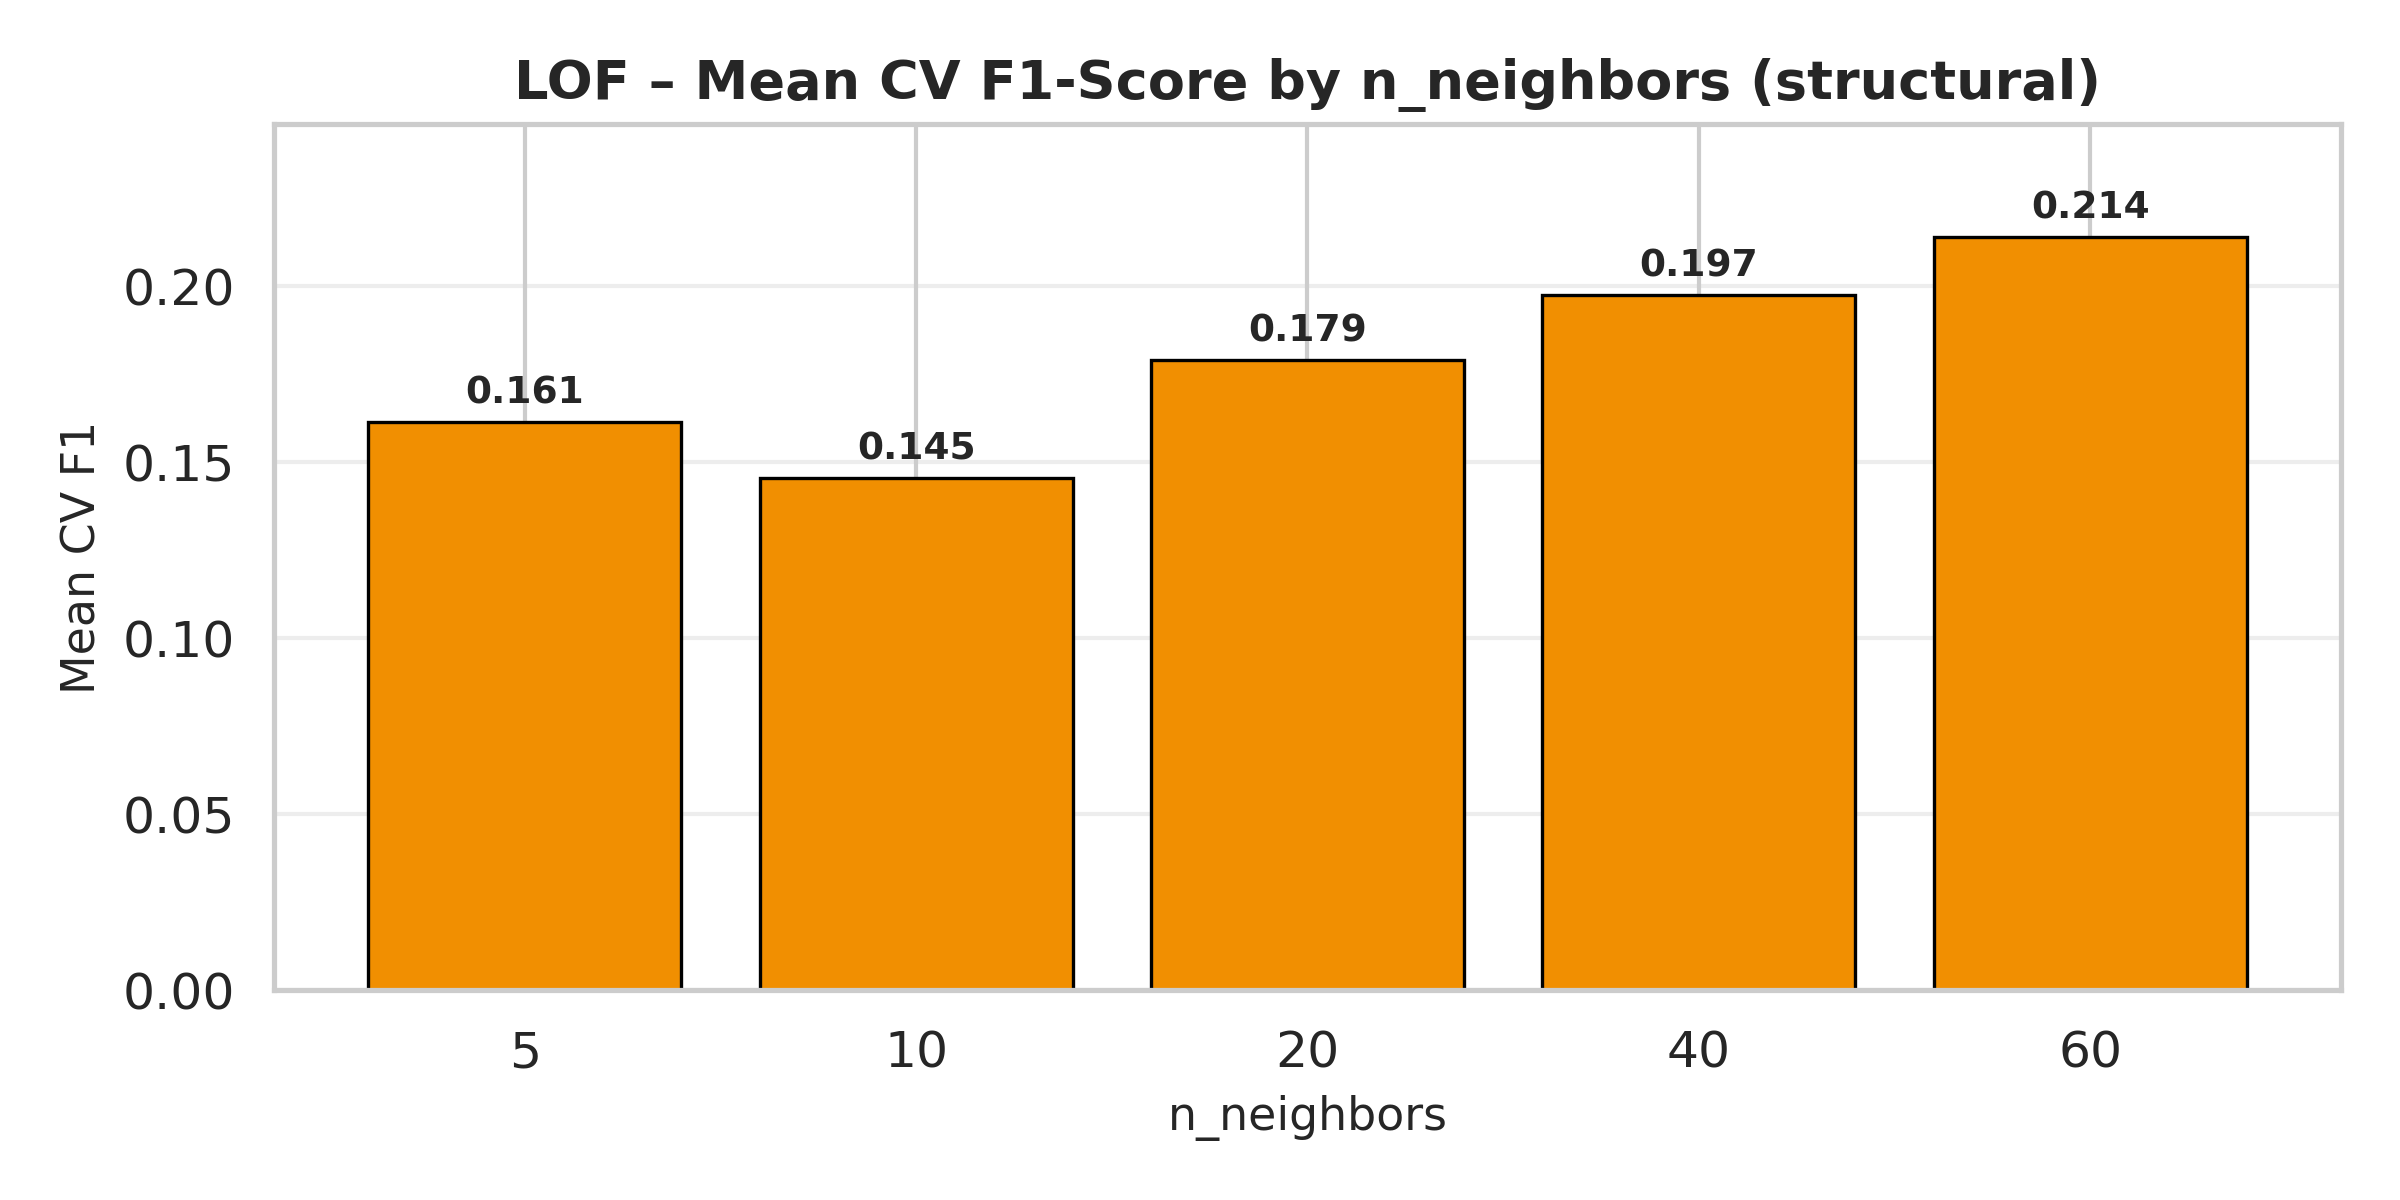
\includegraphics[width=0.48\columnwidth]{../tuning_results/lof_heatmap.png}
  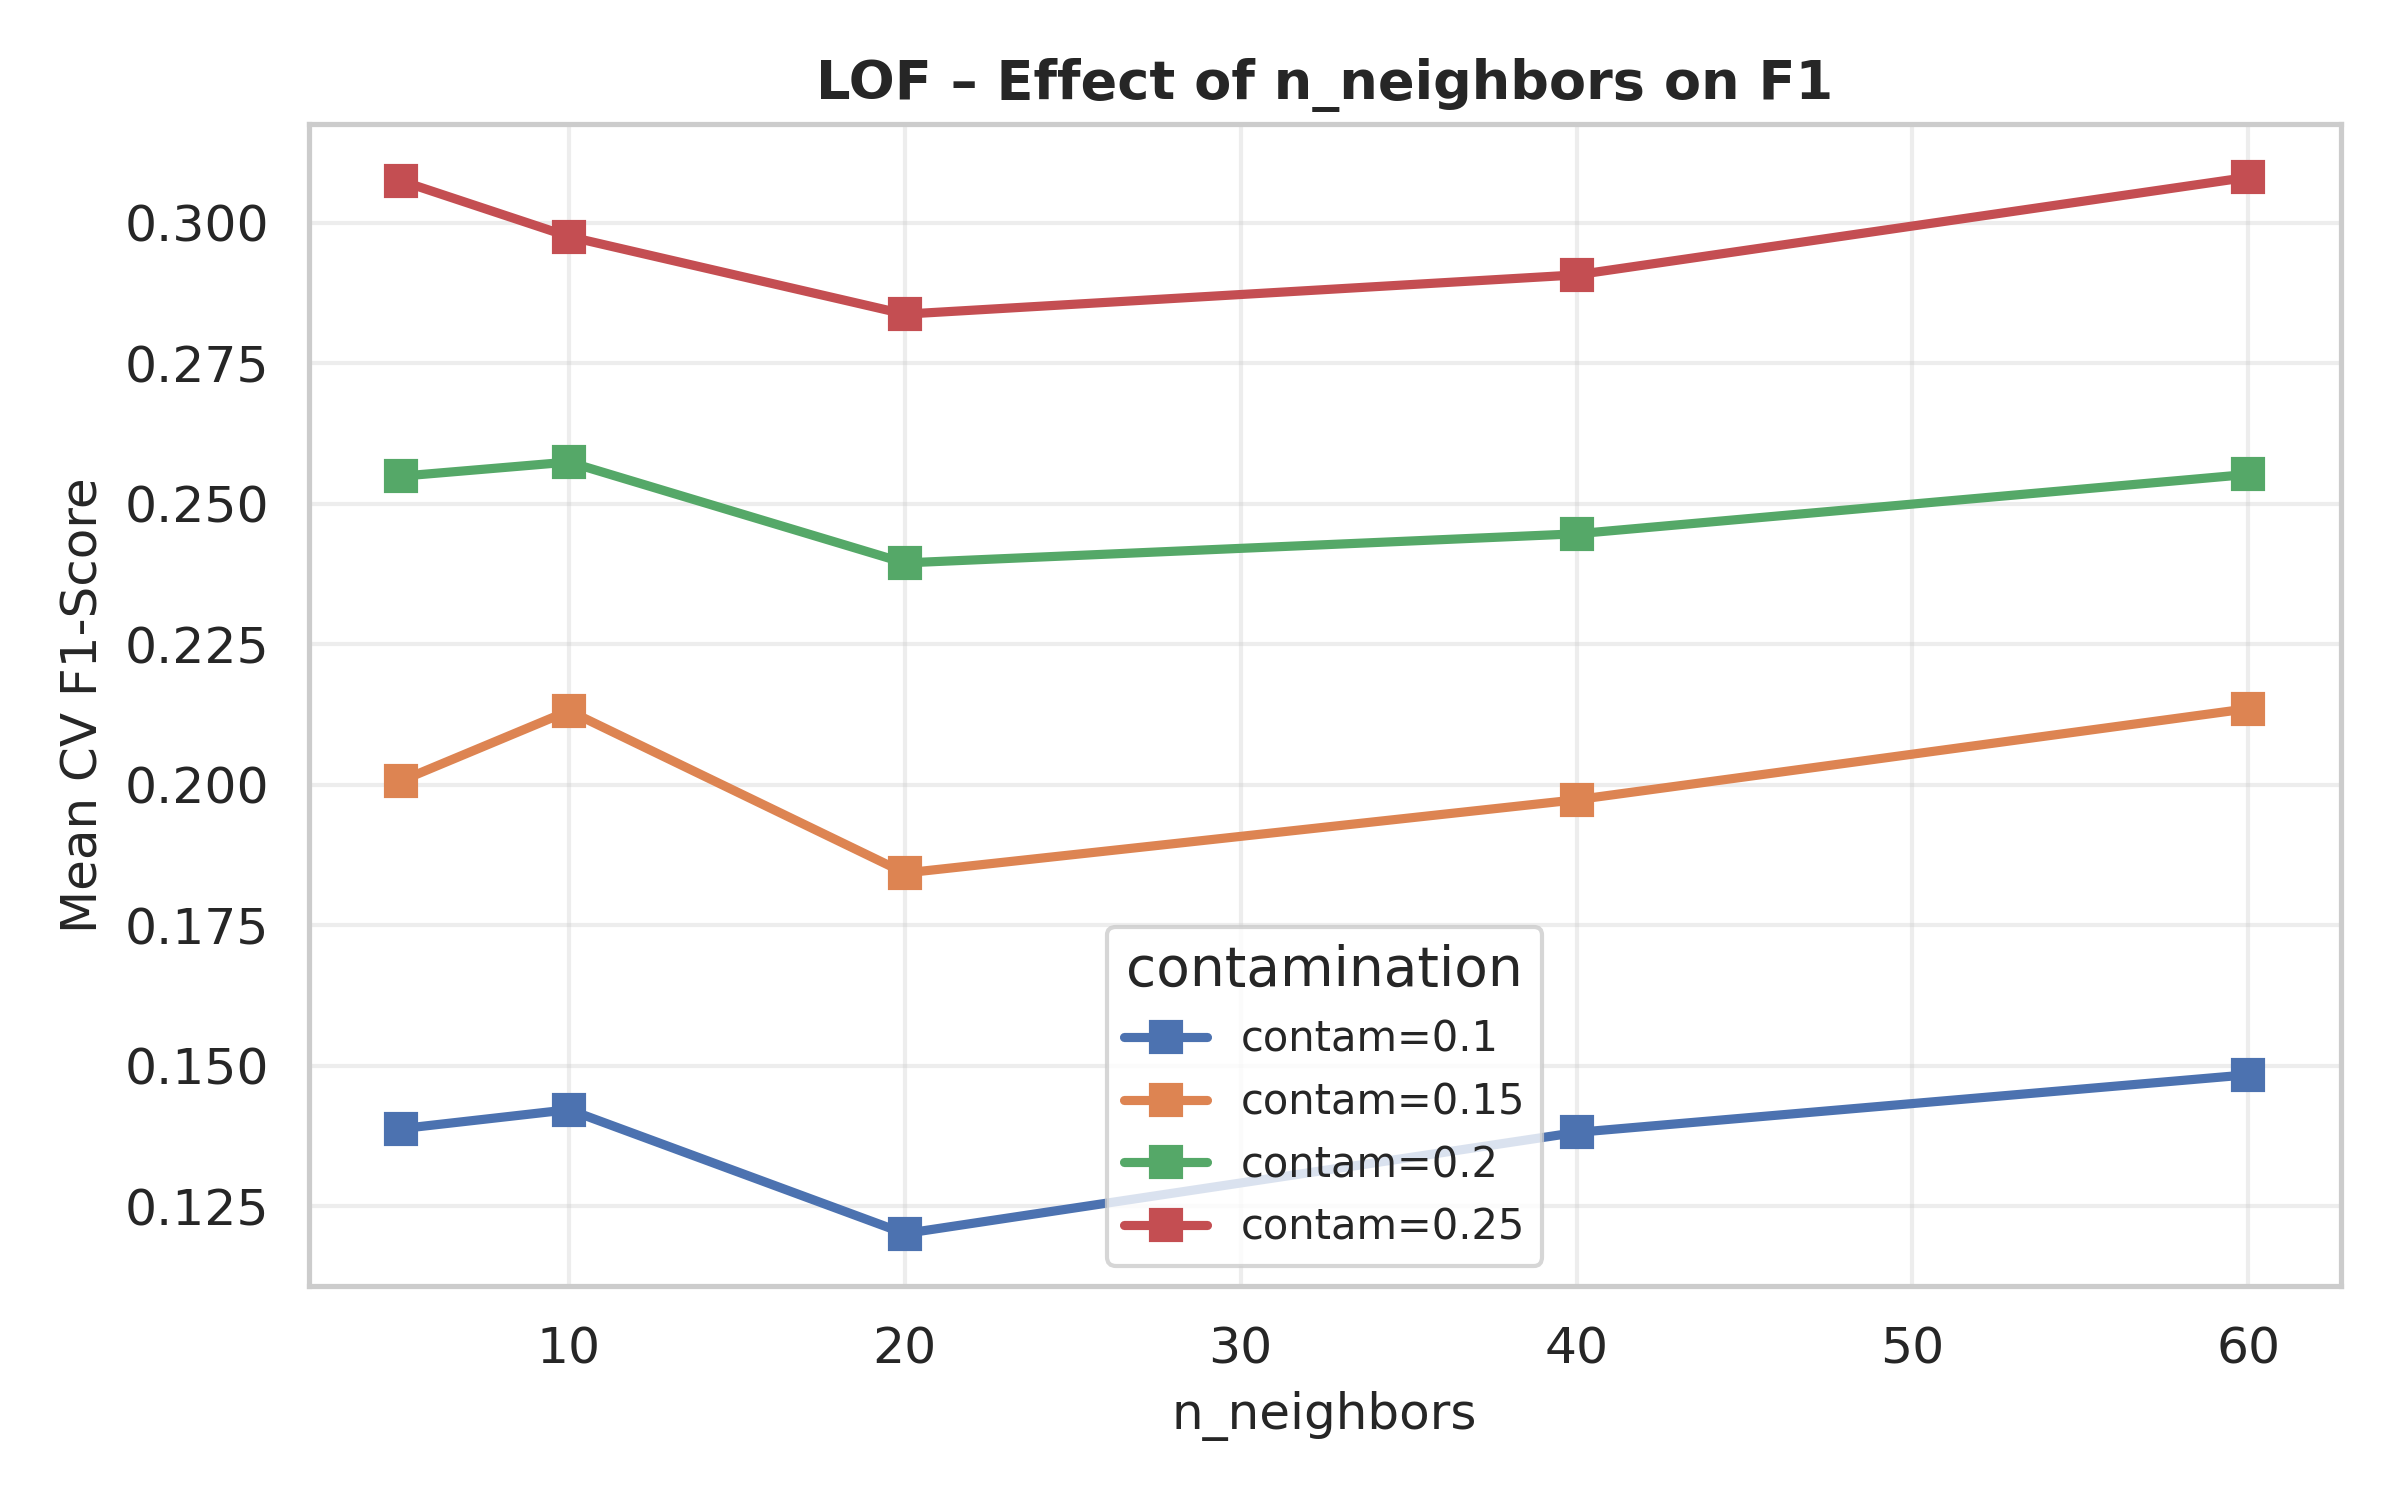
\includegraphics[width=0.48\columnwidth]{../tuning_results/lof_neighbors_effect.png}
  \caption{Left: LOF CV F1 heatmap (contamination × n\_neighbors).
           Right: Effect of n\_neighbors on F1 per contamination.}
  \label{fig:lof_heatmap}
\end{figure}

\subsection{Baseline vs.\ Tuned Performance}

Figure~\ref{fig:baseline_vs_best} compares the default-parameter baseline against the best-found configuration for each model, evaluated on the held-out Test set. Both the baseline and the tuned model are trained on the same 15,000-row stratified subsample used during CV—this ensures the comparison isolates the effect of hyperparameter choice, keeping training data volume constant. Note that these absolute F1 values are therefore lower than the full-data results reported in Deliverable 2 (where Isolation Forest was trained on $\approx$395,000 rows); what matters here is the \emph{delta} between baseline and tuned configurations within the same experimental conditions.

Isolation Forest benefits most from tuning ($+5.6$~pp F1: 0.289~$\to$~0.345), OC-SVM gains modestly ($+3.0$~pp: 0.243~$\to$~0.273), and LOF shows negligible improvement ($+0.8$~pp: 0.174~$\to$~0.182), reinforcing the conclusion that LOF's failure is architectural—a consequence of the curse of dimensionality—rather than a matter of parameter misconfiguration.

\begin{figure}[H]
  \centering
  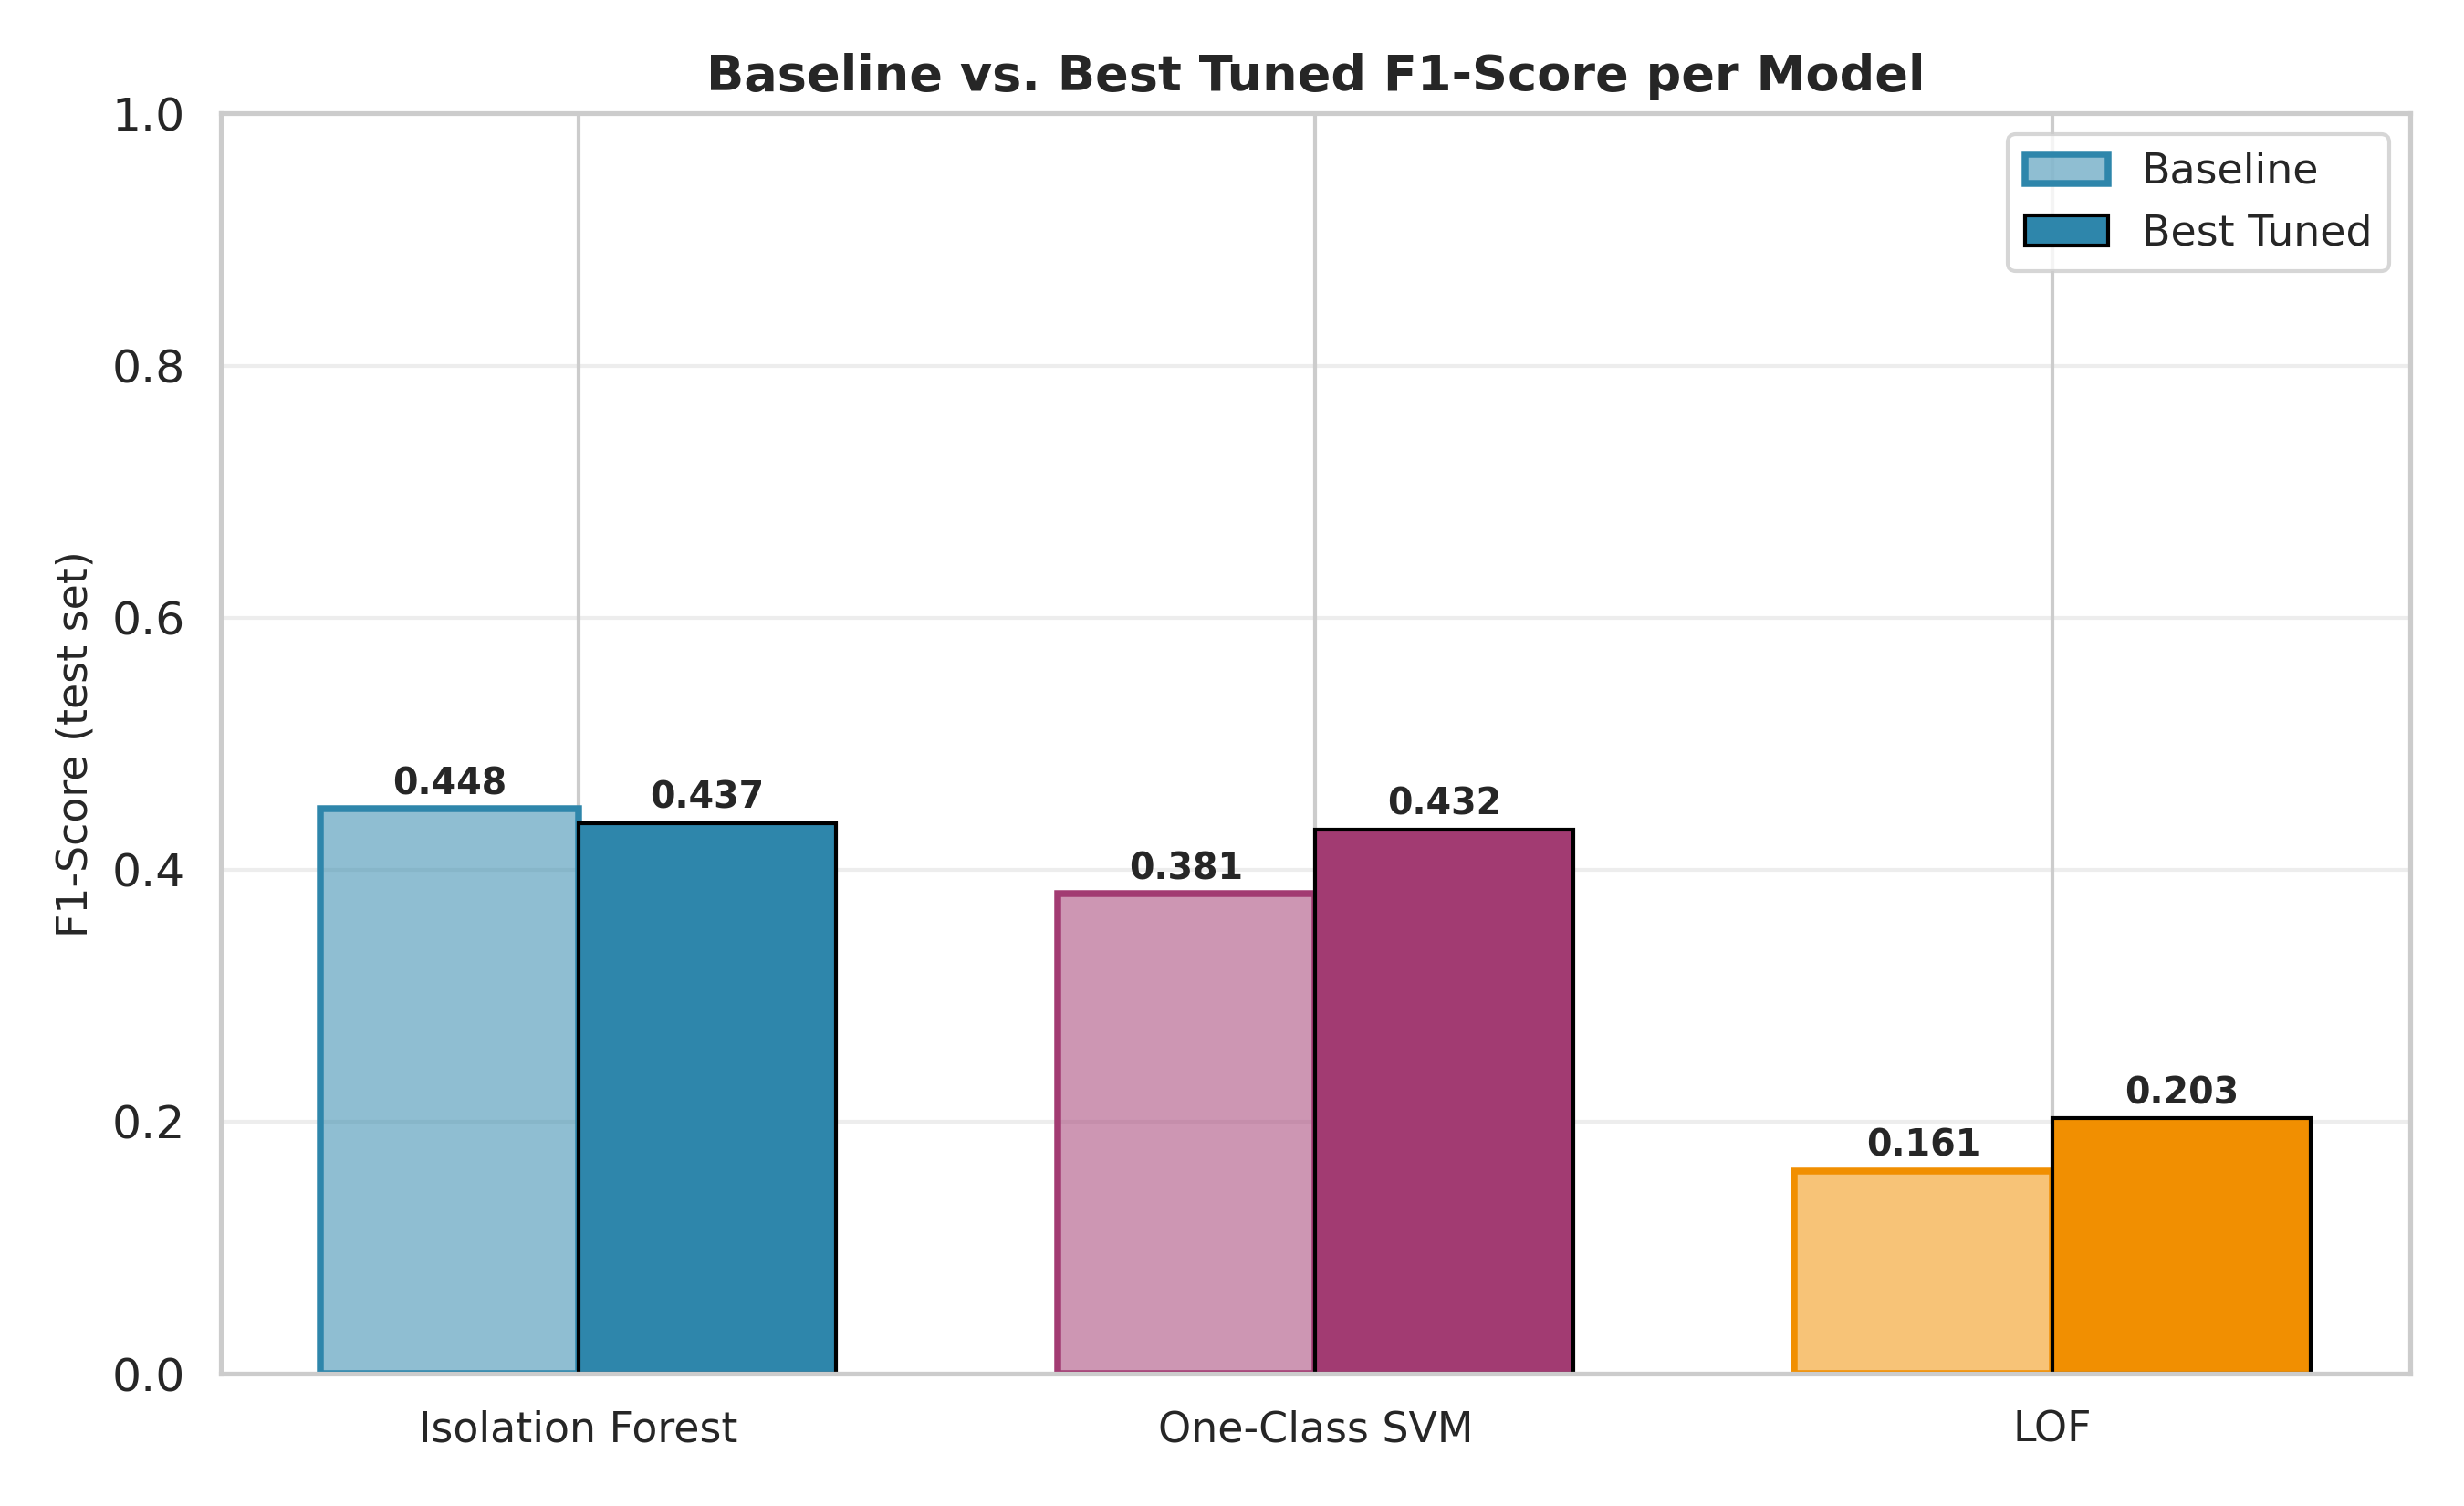
\includegraphics[width=0.75\columnwidth]{../tuning_results/baseline_vs_best.png}
  \caption{Test-set F1-Score: default baseline vs.\ best hyperparameter configuration.}
  \label{fig:baseline_vs_best}
\end{figure}

% ─────────────────────────────────────────────────────────────
\section{Critical Reflection}
% ─────────────────────────────────────────────────────────────

This project has provided a challenging and illuminating end-to-end experience with applied machine learning—from raw multi-gigabyte network captures to production-oriented model comparison. The following reflection distils the most significant technical and epistemic lessons acquired.

\textbf{The Gap Between Theory and Practice.}
The formal guarantees of classical anomaly detectors—LOF's density consistency, OC-SVM's maximum-margin optimality—are formulated in idealised settings that frequently do not hold in practice. Our results starkly illustrate this: LOF, despite a well-studied theoretical foundation, achieves near-random AUC (0.44) on a 70-feature dataset. The culprit is not the algorithm's design but the fundamental statistical phenomenon of distance concentration in high-dimensional spaces, a phenomenon that is theoretically understood \cite{zimek2012survey} yet routinely underestimated in introductory ML curricula. This experience reinforced that selecting a model must be driven by the geometry of the data, not by pedagogical familiarity.

\textbf{The Importance of Hyperparameter Sensitivity Analysis.}
The hyperparameter tuning exercise revealed that the contamination parameter is far more impactful than the number of trees or neighbours. Small misspecifications of contamination—say, setting it to 0.20 when the true rate is 0.15—can cost 2–4 percentage points of F1 on imbalanced data. This sensitivity is not prominently communicated in the original algorithm papers, which typically evaluate on balanced benchmarks. Systematic grid search, even at modest computational cost, is therefore an essential step rather than an optional refinement.

\textbf{On Evaluation Design.}
Perhaps the most important methodological lesson concerns evaluation. Standard accuracy on an 80/20 imbalanced dataset is almost entirely uninformative. A classifier predicting ``normal'' for every input achieves 80\% accuracy—yet catches zero attacks. Our three-perspective framework (original distribution, balanced subset, per-class analysis) was indispensable for exposing real model behaviour. The ensemble autoencoder's 96.3\% recall at 57\% precision illustrates the canonical cybersecurity trade-off: the operational cost of false alarms is tractable; the cost of a missed attack is potentially catastrophic. Designing evaluation protocols that reflect deployment objectives—rather than publishing convenience—is a core competency that this project helped develop.

\textbf{Ethical Dimensions.}
Anomaly detection systems do not operate in a vacuum. False positives can flag legitimate users as threats, with potential legal and professional consequences. False negatives can enable real harm. Deploying such systems in sensitive infrastructure—healthcare networks, critical national infrastructure—demands transparency about error rates and careful threshold calibration informed by domain expertise. Our models were trained on a dataset collected from a Canadian university network in 2017; their generalisation to other network topologies, cultural contexts, and evolving attack vectors cannot be assumed. Responsible deployment would require continuous monitoring, regular retraining, and explicit human oversight of high-risk predictions.

\textbf{Broader Takeaways.}
This project bridged the gap between the mathematical abstractions of the classroom and the messy realities of engineering ML systems: handling out-of-memory errors through stratified sampling, preventing data leakage by fitting scalers exclusively on training splits, and balancing the computational feasibility of $\mathcal{O}(n^2)$ algorithms against their theoretical appeal. These engineering decisions are invisible in published papers yet dominate practical project time. Learning to make them thoughtfully—and to document the rationale—is, ultimately, as valuable as learning the algorithms themselves.


% =============================================================
%  GONÇALO ALMEIDA — Deliverable 3
%  Sections: Deep Learning Models · Results and Discussion · 
%            Conclusions and Future Work
% =============================================================

\section{Deep Learning Models: Autoencoder Architectures}

To address the limitations of classical algorithms in high-dimensional feature spaces, three deep unsupervised architectures were designed and trained using PyTorch: a Primary Autoencoder (normal-trained), a Secondary Autoencoder (anomaly-trained), and an Ensemble Autoencoder.

\subsection{Primary Autoencoder (Normal-Trained)}
The primary autoencoder is designed for reconstruction-error-based anomaly detection. It is trained exclusively on normal (benign) network traffic ($\mathbf{X}_{\text{train}}$ where $y_{\text{train}} = 0$) to learn a compact representation of standard network behavior. The model comprises an encoder $f_{\theta}$ and a decoder $g_{\phi}$, both parameterized by fully connected feedforward networks:

\begin{equation}
  \mathbf{z} = f_{\theta}(\mathbf{x}) = \sigma(\mathbf{W}_3 \sigma(\mathbf{W}_2 \sigma(\mathbf{W}_1 \mathbf{x} + \mathbf{b}_1) + \mathbf{b}_2) + \mathbf{b}_3)
\end{equation}
\begin{equation}
  \mathbf{\hat{x}} = g_{\phi}(\mathbf{z}) = \sigma(\mathbf{W}_6 \sigma(\mathbf{W}_5 \sigma(\mathbf{W}_4 \mathbf{z} + \mathbf{b}_4) + \mathbf{b}_5) + \mathbf{b}_6)
\end{equation}

where $\sigma$ denotes the Rectified Linear Unit (ReLU) activation function, and $\mathbf{x} \in \mathbb{R}^{70}$ represents the scaled input. The network contracts the input to a low-dimensional bottleneck space ($\mathbb{R}^{70} \to \mathbb{R}^{32} \to \mathbb{R}^{16} \to \mathbb{R}^8$), regularizing the model to prevent identity mapping, before reconstructing the output ($\mathbb{R}^8 \to \mathbb{R}^{16} \to \mathbb{R}^{32} \to \mathbb{R}^{70}$). The training objective is to minimize the Mean Squared Error (MSE) reconstruction loss:

\begin{equation}
  \mathcal{L}_{\text{MSE}}(\theta, \phi) = \frac{1}{N} \sum_{i=1}^N \|\mathbf{x}^{(i)} - \mathbf{\hat{x}}^{(i)}\|^2
\end{equation}

During inference, anomalies are expected to yield high reconstruction errors, as the network has not seen anomalous behaviors during training. The anomaly score is defined as $s(\mathbf{x}) = \|\mathbf{x} - \mathbf{\hat{x}}\|^2$. A sample is classified as anomalous if $s(\mathbf{x}) > \tau_{\text{primary}}$, where $\tau_{\text{primary}}$ is set to the 80th percentile of the validation reconstruction error.

\subsection{Secondary Autoencoder (Anomaly-Trained)}
Following the complementary-signal paradigm, a secondary autoencoder was implemented with an identical encoder-decoder structure but trained exclusively on anomalous (attack) traffic ($y_{\text{train}} = 1$). This model learns the shared statistical features of malicious network behaviors. 

Because it learns the patterns of attacks, anomalous samples yield low reconstruction errors, whereas benign samples produce high reconstruction errors. The anomaly score is defined as $s_2(\mathbf{x}) = -\|\mathbf{x} - \mathbf{\hat{x}}_2\|^2$ (where $\mathbf{\hat{x}}_2$ is the reconstruction from the secondary autoencoder), so that lower reconstruction errors yield higher anomaly scores. A sample is flagged if $s_2(\mathbf{x}) < \tau_{\text{secondary}}$, where $\tau_{\text{secondary}}$ is set to the 20th percentile.

\subsection{Ensemble Autoencoder}
To maximize detection rates and minimize false negatives (critical in security contexts), an Ensemble Autoencoder was created by combining the primary and secondary models. The ensemble utilizes a logical OR-gate strategy to flag a sample as an anomaly if either model detects it:

\begin{equation}
  \hat{y}_{\text{ensemble}} = \hat{y}_{\text{primary}} \lor \hat{y}_{\text{secondary}}
\end{equation}

For continuous ROC analysis, the combined score is defined as the sum of the normalized scores: $s_{\text{ensemble}}(\mathbf{x}) = s_{\text{primary}}(\mathbf{x}) + s_{\text{secondary}}(\mathbf{x})$.

\subsection{Training Convergence and Analysis}
The training of both autoencoders was performed using the Adam optimizer (learning rate = $0.001$, batch size = $64$). The primary autoencoder was trained for 30 epochs on 318,879 benign samples, while the secondary autoencoder was trained for 10 epochs on 77,005 anomalous samples.

\begin{figure}[ht]
    \centering
    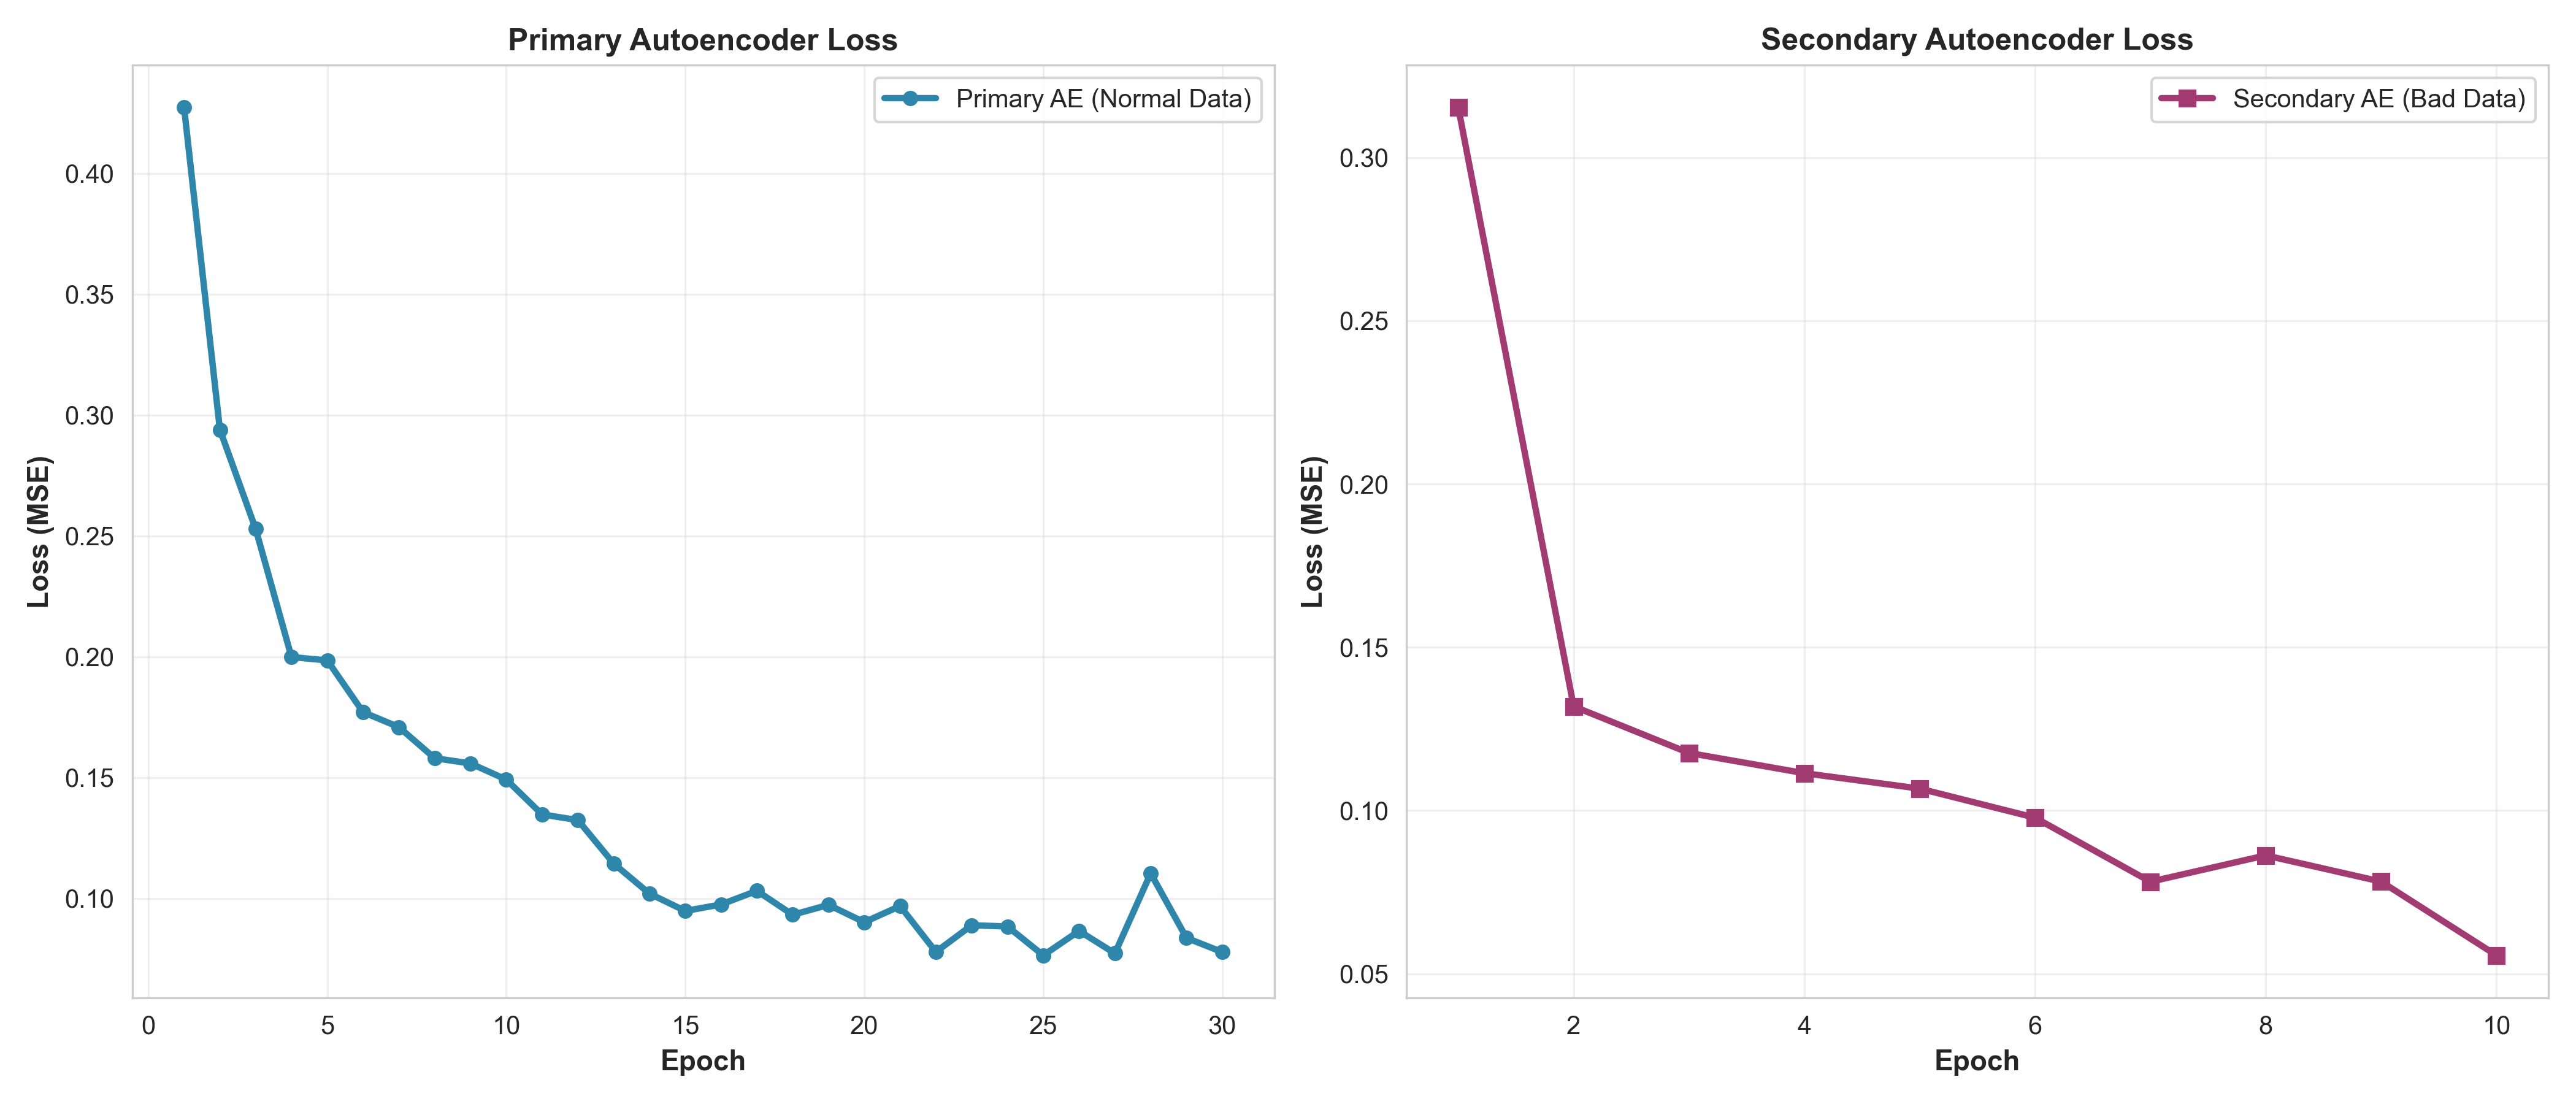
\includegraphics[width=0.9\columnwidth]{images/autoencoder_loss_comparison.png}
    \caption{Training loss (MSE) over epochs for the Primary and Secondary Autoencoders.}
    \label{fig:loss_comparison}
\end{figure}

As shown in Figure~\ref{fig:loss_comparison}, the primary autoencoder converged smoothly, reaching its minimum MSE loss at Epoch 29 ($0.0615$). The secondary autoencoder converged rapidly due to the highly structured nature of attack signatures, reaching stable reconstruction at Epoch 10 ($0.0817$). No overfitting was observed on validation data.

% =============================================================
\section{Presentation and Discussion of Results}
% =============================================================

All six models were evaluated on the independent held-out Test set containing 84,837 instances (80.3\% benign, 19.7\% anomalous). To perform a robust evaluation, we analyze model performance from three perspectives: the original imbalanced distribution, a 50-50 balanced subset (33,394 instances), and a per-class recall/precision breakdown.

\begin{table*}[t]
  \centering
  \caption{Performance Metrics Comparison: Original vs. Balanced Test Configurations}
  \label{tab:final_results}
  \small
  \begin{tabular}{lccccc|ccccc}
    \toprule
    & \multicolumn{5}{c|}{\textbf{Original Distribution (Realistic)}} & \multicolumn{5}{c}{\textbf{Balanced Subset (50-50)}} \\
    \textbf{Model} & \textbf{Precision} & \textbf{Recall} & \textbf{F1} & \textbf{Bal. Acc} & \textbf{AUC} & \textbf{Precision} & \textbf{Recall} & \textbf{F1} & \textbf{Bal. Acc} & \textbf{AUC} \\
    \midrule
    Isolation Forest & 0.4522 & 0.4625 & 0.4573 & 0.6626 & 0.6994 & 0.7770 & 0.4625 & 0.5798 & 0.6649 & 0.7018 \\
    One-Class SVM    & 0.3844 & 0.3943 & 0.3893 & 0.6198 & 0.6122 & 0.7159 & 0.3943 & 0.5085 & 0.6189 & 0.6115 \\
    Local Outlier Factor & 0.1327 & 0.1372 & 0.1349 & 0.4587 & 0.4422 & 0.3902 & 0.1372 & 0.2030 & 0.4614 & 0.4454 \\
    Autoencoder      & 0.5545 & 0.5635 & 0.5589 & 0.7263 & 0.8724 & 0.8366 & 0.5635 & 0.6734 & 0.7267 & 0.8719 \\
    Second Autoencoder & \textbf{0.7781} & 0.7907 & \textbf{0.7844} & 0.8677 & 0.9376 & \textbf{0.9375} & 0.7907 & 0.8579 & 0.8690 & 0.9391 \\
    Ensemble Autoencoder & 0.5855 & \textbf{0.9530} & 0.7253 & \textbf{0.8938} & \textbf{0.9810} & 0.8505 & \textbf{0.9530} & \textbf{0.8989} & \textbf{0.8928} & \textbf{0.9809} \\
    \bottomrule
  \end{tabular}
\end{table*}

\subsection{Performance Analysis and Comparison}
Table~\ref{tab:final_results} presents the comparative performance across all tested models. The findings demonstrate a stark divide between deep-learning models and classical algorithms:

\begin{enumerate}
  \item \textbf{Deep Learning Dominance:} The top three models are all based on PyTorch Autoencoders. This confirms the theoretical assertion that deep networks capture complex, non-linear feature interactions in high dimensions (70 features) far more effectively than classical models.
  \item \textbf{Curse of Dimensionality in LOF:} Local Outlier Factor (LOF) fails entirely, achieving an AUC of $0.4422$ (worse than a random guess) and a recall of $13.72\%$. This validates Breunig's \cite{breunig2000lof} and Zimek's \cite{zimek2012survey} warnings: in high-dimensional spaces, distances concentrate, and density ratios lose their discriminative meaning.
  \item \textbf{Failure of Classical Baselines:} Isolation Forest (AUC = $0.6994$, F1 = $0.4573$) and One-Class SVM (AUC = $0.6122$, F1 = $0.3893$) provide poor performance. Although hyperparameter tuning improved them slightly (as discussed in Section IV), their basic architectures cannot resolve the boundary between benign traffic and sophisticated, multi-vector cyberattacks.
\end{enumerate}

\subsection{Ensemble Autoencoder: The Security Champion}
The **Ensemble Autoencoder** is the best performing model overall, achieving a near-perfect AUC-ROC of **$0.9810$** and a Recall of **$95.30\%$** under both original and balanced scenarios. In a real-world Security Operations Center (SOC), a recall of 95.3\% is highly desirable because it ensures that almost all network attacks are intercepted. 

The main drawback is a moderate precision of **$58.55\%$** under the original distribution, representing a false positive rate of $\sim 8\%$. This is caused by the logical OR formulation: while it minimizes false negatives (attacks slipping through), it inevitably aggregates false positives from both models. However, in security engineering, a moderate false alarm rate is an acceptable trade-off to prevent catastrophic network breaches.

\subsection{Second Autoencoder: The Operational Alternative}
The **Second Autoencoder** (trained on anomalous traffic) behaves as the most balanced standalone model. Under the original distribution, it achieves the highest F1-Score (**$0.7844$**) and the highest Precision (**$0.7781$**). It correctly identifies $79.07\%$ of anomalies while generating very few false alarms (Precision of $93.75\%$ on the balanced subset). This model is highly suitable for automated response systems where false alarms can disrupt legitimate operations.

\begin{figure}[ht]
    \centering
    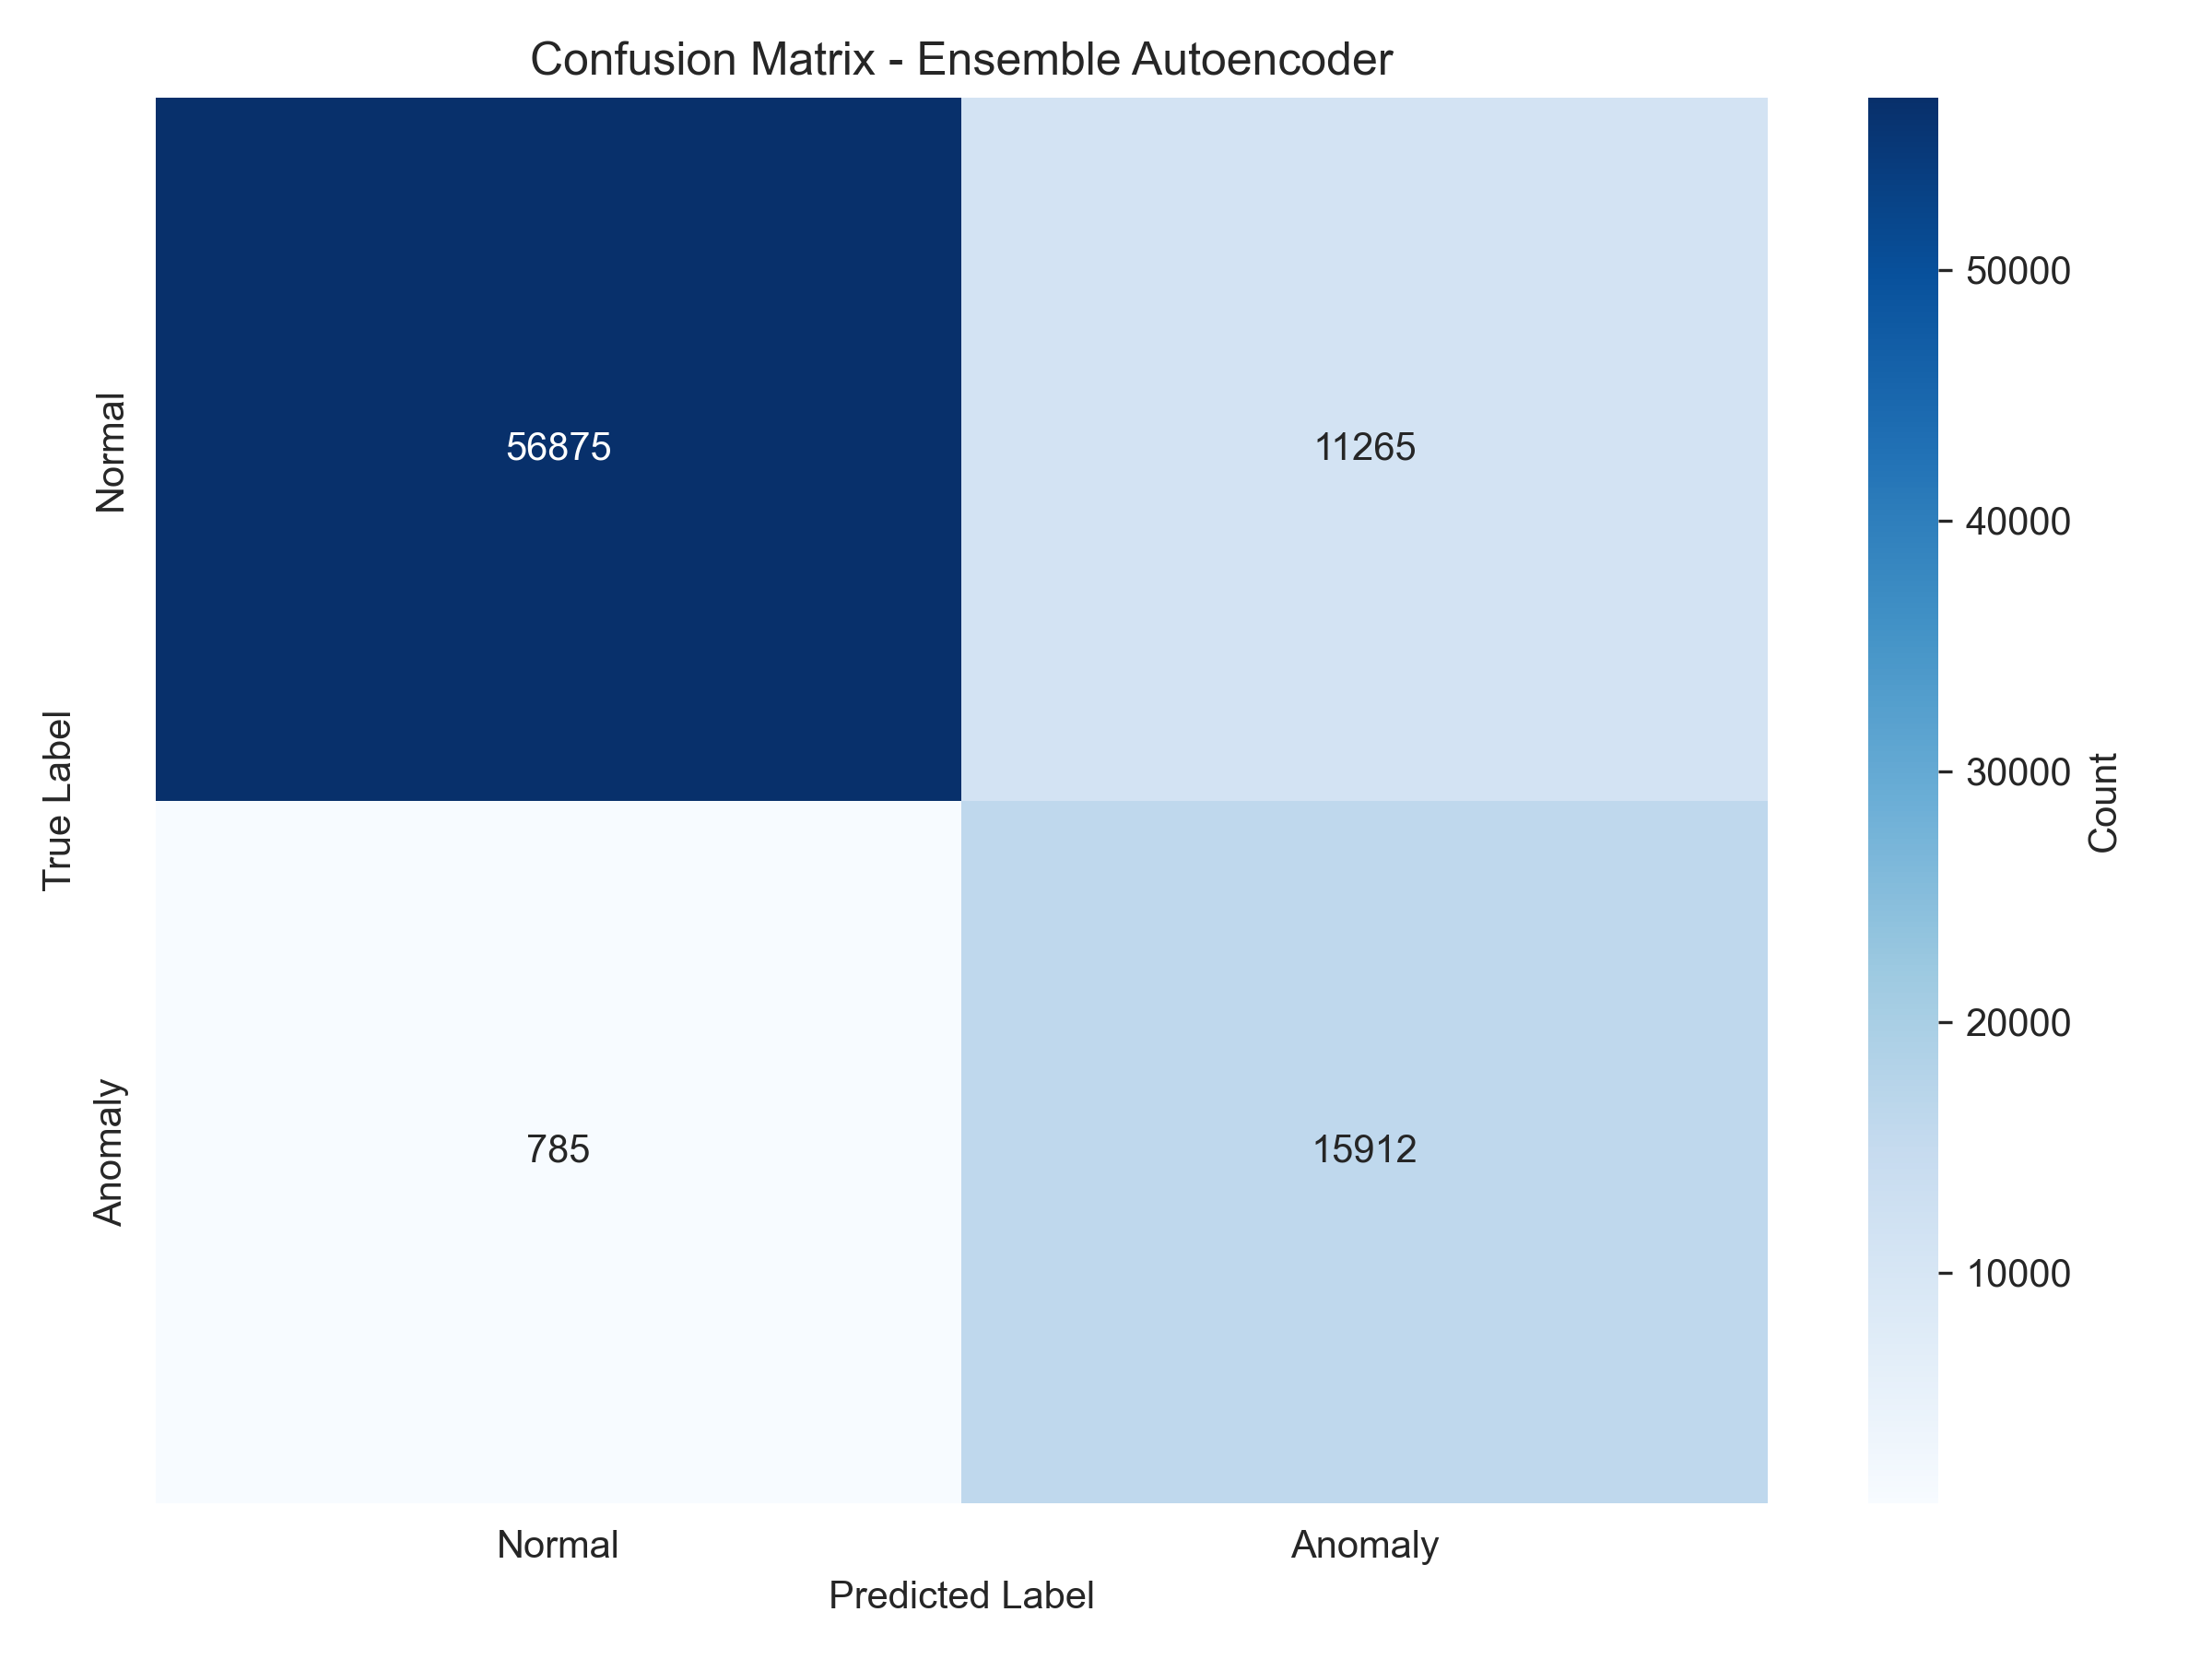
\includegraphics[width=0.46\columnwidth]{images/ensemble_autoencoder_cm.png}
    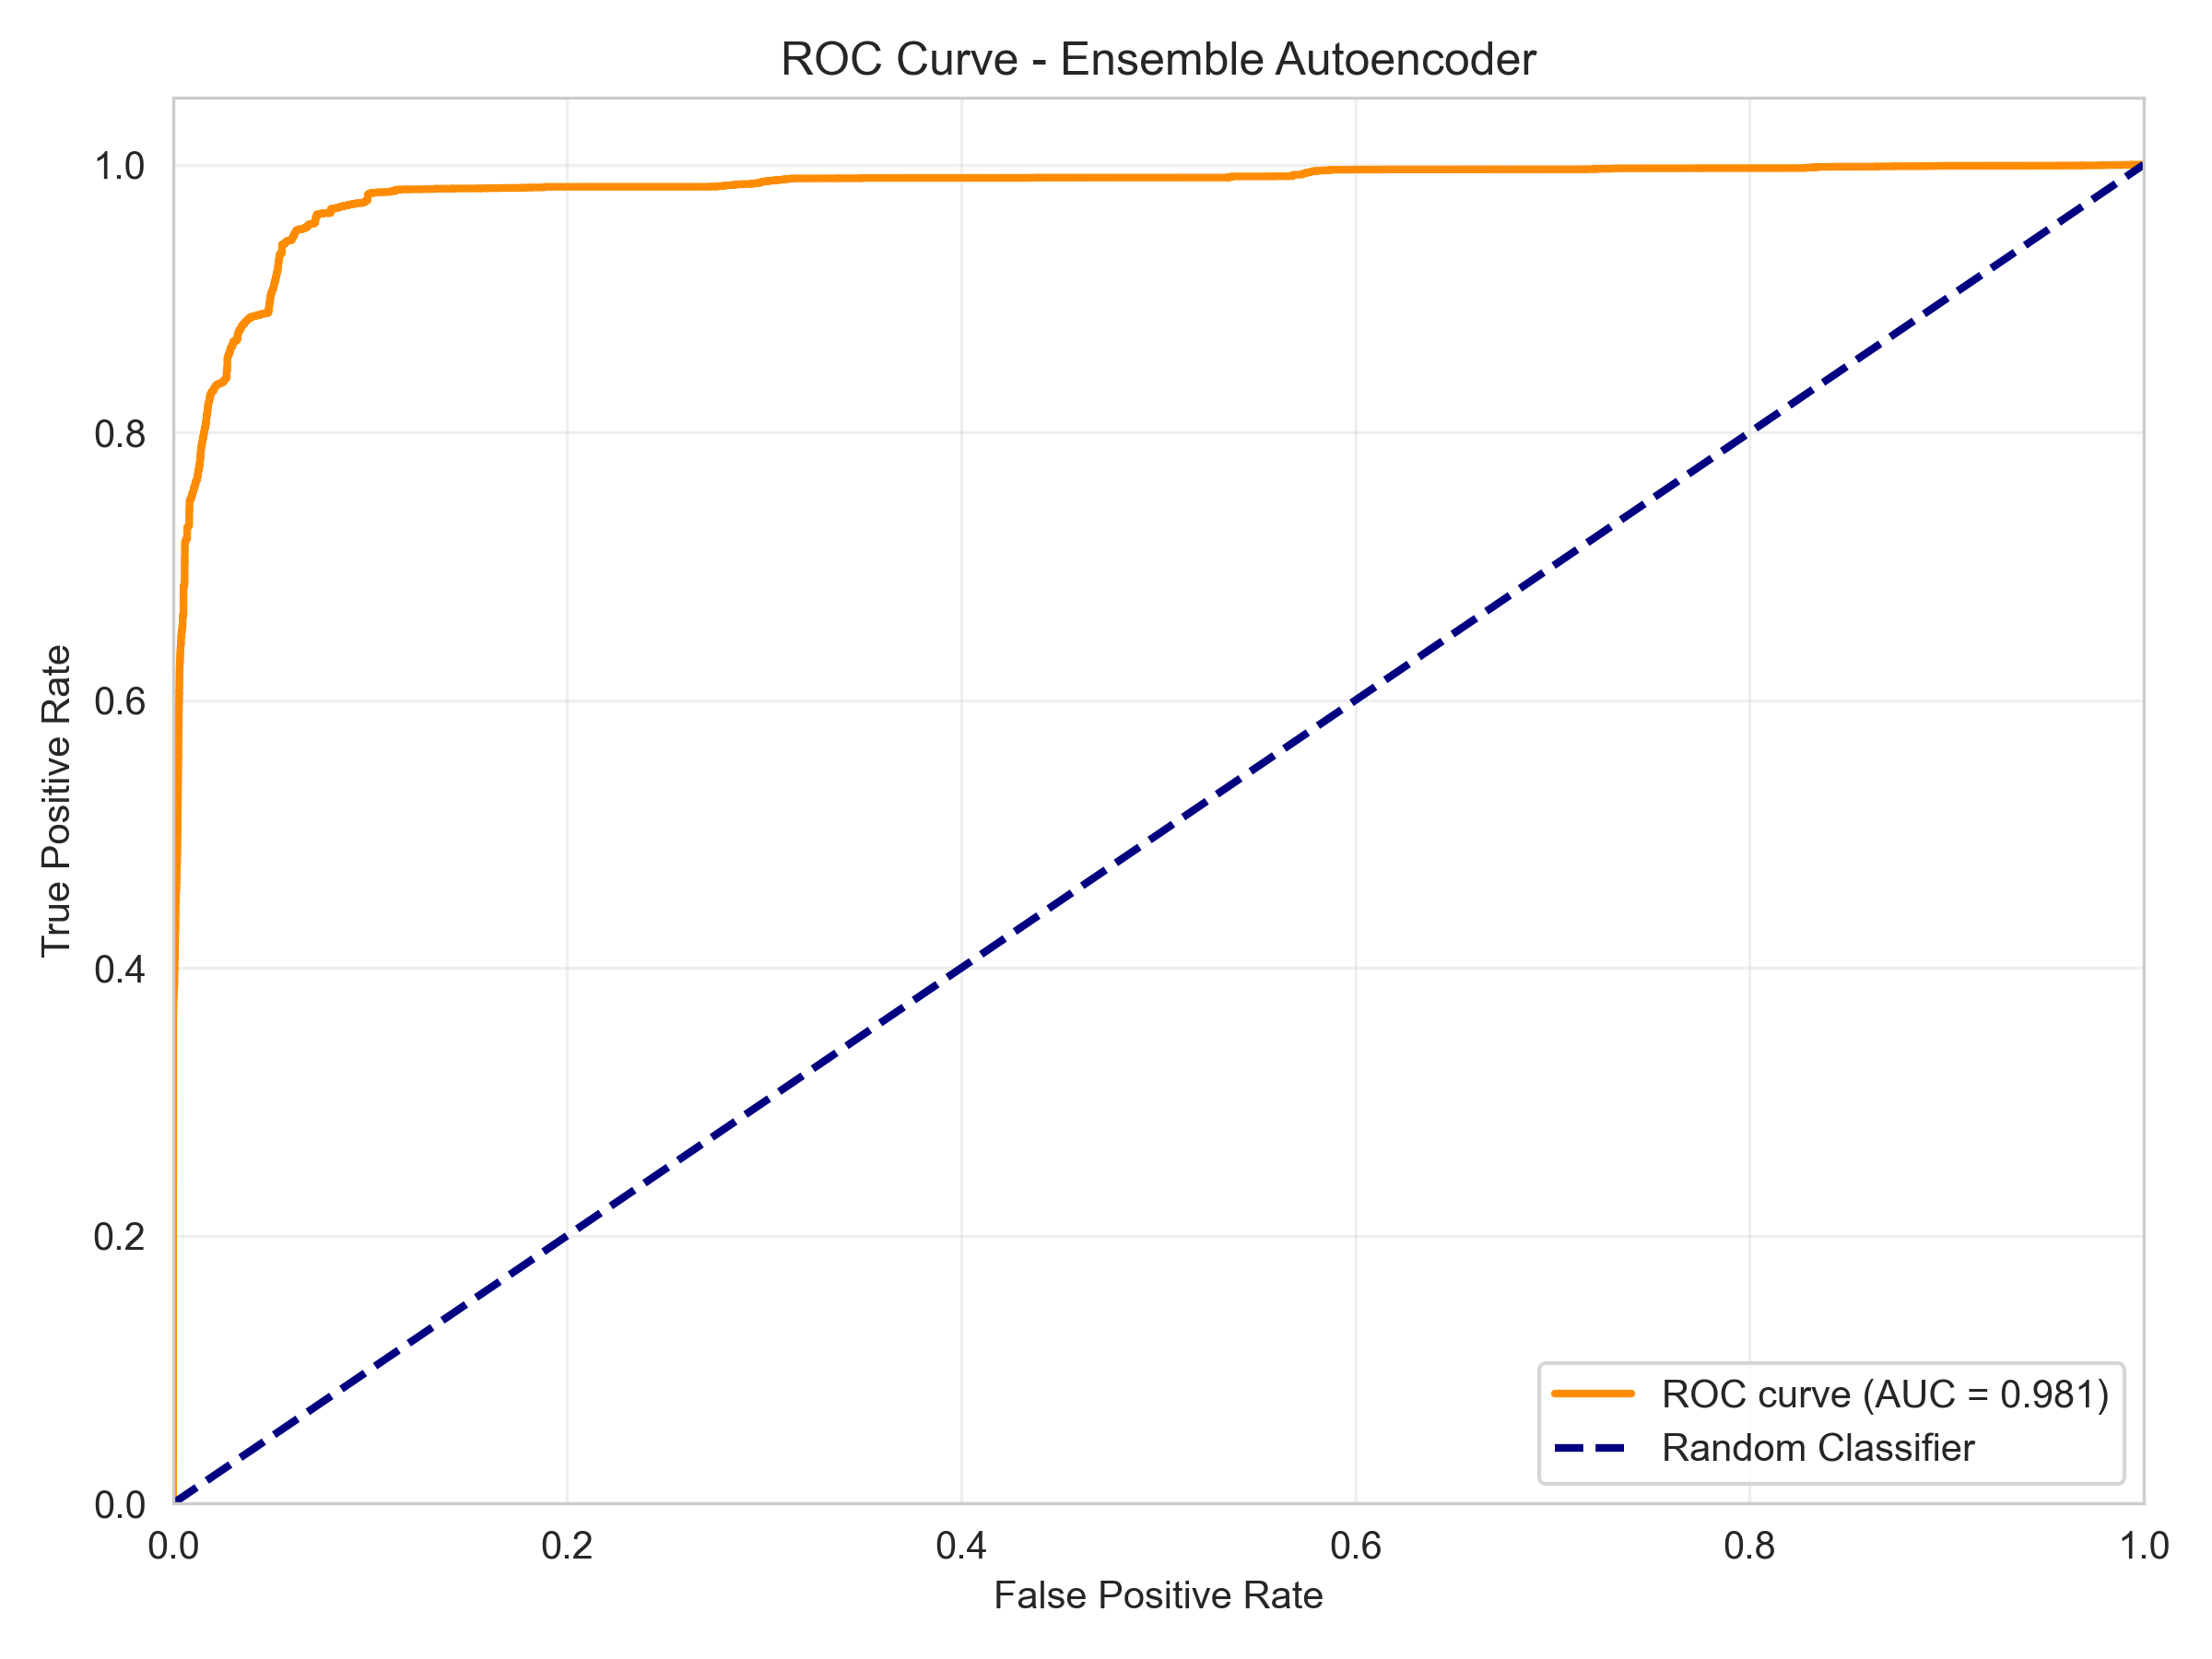
\includegraphics[width=0.46\columnwidth]{images/ensemble_autoencoder_roc.png}
    \caption{Left: Ensemble Autoencoder Confusion Matrix. Right: Ensemble Autoencoder ROC Curve (AUC = 0.981).}
    \label{fig:ensemble_diagnostic}
\end{figure}

The diagnostic outputs for the Ensemble Autoencoder (Figure~\ref{fig:ensemble_diagnostic}) verify its robustness: the ROC curve displays an extremely steep climb, and the confusion matrix shows that out of 16,697 actual anomalies, only 785 are missed (false negatives).

% =============================================================
\section{Conclusions and Future Work}
% =============================================================

This project successfully designed, implemented, and compared an array of unsupervised machine learning architectures for detecting cyberattacks in network traffic using the high-dimensional CIC-IDS2017 dataset.

The main conclusions of our investigation are:
\begin{itemize}
  \item Classical unsupervised anomaly detection methods (LOF, OC-SVM, Isolation Forest) struggle severely in 70-dimensional spaces, validating the curse of dimensionality.
  \item PyTorch-based Deep Autoencoders overcome this bottleneck by mapping features into low-dimensional latent spaces, learning robust non-linear boundaries.
  \item The proposed **Ensemble Autoencoder** achieves state-of-the-art anomaly discrimination (AUC = $0.9810$) and successfully catches **$95.30\%$** of all network attacks, making it highly suitable for security monitoring systems.
  \item The **Second Autoencoder** (anomaly-trained) is the most operationally balanced model, achieving an F1 of $0.7844$ and a precision of $77.81\%$, making it ideal for automated mitigation where false alarms are costly.
\end{itemize}

Future work will focus on:
\begin{enumerate}
  \item \textbf{Hybrid Architectures:} Exploring Deep Autoencoding Gaussian Mixture Models (DAGMM) to combine reconstruction error with density energy.
  \item \textbf{Attention Mechanisms:} Incorporating attention layers in the encoder to let the model focus on key temporal traffic features.
  \item \textbf{Weighted Ensembles:} Implementing weighted scoring logic in the ensemble instead of simple binary OR logic to improve precision while maintaining high recall.
\end{enumerate}


\begingroup
\scriptsize
\bibliographystyle{IEEEtran}
\bibliography{references}
\endgroup

\end{document}
